%\documentclass{sbmlpkgspec}
\documentclass[draftspec]{sbmlpkgspec}

\hypersetup{
    pdfauthor = {Brett G. Oliver and Frank T. Bergmann and Sarah Keating and Matthias Konig}
}

%\frontNotice{\centering This is Release Candidate 7 of the ``fbc'' package Version 2, Release 1 and not a normative document. Please send feedback to the Package Working Group mailing list at sbml-flux@lists.sourceforge.net. The official Version 1 Release 1 specification can be found here: \url{http://identifiers.org/combine.specifications/sbml.level-3.version-1.fbc.version-1.release-1}}

\begin{document}

\packageTitle{SBML Level 3 Package: Flux Balance Constraints (`fbc')}
\packageVersion{Version 3, Release 1, Release Candidate 2}
\packageVersionDate{\today}%September 12, 2015
\packageGeneralURL{http://sbml.org/Documents/Specifications/SBML_Level_3/Packages/Flux_Balance_Constraints_(flux)}
%\packageThisVersionURL{http://identifiers.org/combine.specifications/sbml.level-3.version-1.fbc.version-1.release-1}
\packageThisVersionURL{http://identifiers.org/combine.specifications/sbml.level-3.version-1.fbc.version-3.release-1}

\author{%
\begin{tabular}{c>{\hspace{20pt}}c}
Brett G. Olivier PhD & Frank T. Bergmann PhD\\[0.25em]
\mailto{b.g.olivier@vu.nl} & \mailto{fbergmann@caltech.edu}\\[0.25em]
Systems Biology Lab, AIMMS & Computing and Mathematical Sciences\\
Vrije Universiteit Amsterdam & California Institute of Technology\\
Amsterdam, NH, The Netherlands & Pasadena, CA, US\\
 & \\
Sarah Keating PhD & Matthias K\"{o}nig PhD \\[0.25em]
\mailto{s.keating@ucl.ac.uk} & \mailto{konigmatt@googlemail.com} \\[0.25em]
Research Software Development Group & Institute for Theoretical Biology\\
University College London & Humboldt Universit\"{a}t zu Berlin \\
London, UK & Berlin, DE \\
\end{tabular}
}

\renewcommand\graphicspath{{logos}}

\newcommand{\ListOfFluxBounds}{\defRef{ListOfFluxBounds}{listoffluxbounds-class}}
\newcommand{\FluxBound}{\defRef{FluxBound}{fluxbound-class}}
\newcommand{\ListOfObjectives}{\defRef{ListOfObjectives}{listofobjectives-class}}
\newcommand{\Objective}{\defRef{Objective}{objective-class}}
\newcommand{\ListOfFluxObjectives}{\defRef{ListOfFluxObjectives}{listoffluxobjectives-class}}
\newcommand{\FluxObjective}{\defRef{FluxObjective}{fluxobjective-class}}
\newcommand{\ListOfGeneProducts}{\defRef{ListOfGeneProducts}{listofgeneproducts-class}}
\newcommand{\GeneProduct}{\defRef{GeneProduct}{geneproduct-class}}
\newcommand{\ListOfGeneProteinAssociations}{\defRef{ListOfGeneProteinAssociations}{listofgeneproteinassociations-class}}
\newcommand{\GeneProductAssociation}{\defRef{GeneProductAssociation}{geneproductassociation-class}}
\newcommand{\Association}{\defRef{\textit{Association}}{association-class}}
\newcommand{\GeneProductRef}{\defRef{GeneProductRef}{geneproductref-class}}
\newcommand{\GeneAnd}{\defRef{And}{and-class}}
\newcommand{\GeneOr}{\defRef{Or}{or-class}}
% new in v3
\newcommand{\ListOfUserDefinedConstraints}{\defRef{ListOfUserDefinedConstraints}{listofuserdefinedconstraints-class}}
\newcommand{\UserDefinedConstraint}{\defRef{UserDefinedConstraint}{userdefinedconstraint-class}}
\newcommand{\ListOfUserDefinedConstraintComponents}{\defRef{ListOfUserDefinedConstraintComponents}{listofuserdefinedconstraintcomponents-class}}
\newcommand{\UserDefinedConstraintComponent}{\defRef{UserDefinedConstraintComponent}{userdefinedconstraintcomponent-class}}

\newcommand{\ListOfKeyValuePairs}{\defRef{ListOfKeyValuePairs}{listofkeyvaluepairs-class}}
\newcommand{\KeyValuePair}{\defRef{KeyValuePair}{keyvaluepair-class}}

\newcommand{\sbmlthreecore}{SBML Level~3 Version~1 Core\xspace}
\newcommand{\FBC}{\textsf{FBC}\xspace}
\newcommand{\FBCPackage}{\textsf{Flux Balance Constraints} package\xspace}
%Stoichiometric matrix \Nmat
\newcommand{\Nmat}{\ensuremath{\mathbf{N}}}
%Rate vector \vvec
\newcommand{\vvec}{\ensuremath{\mathbf{v}}}
%Flux vector \Jvec
\newcommand{\Jvec}{\ensuremath{\mathbf{J}}}

\newcommand{\sboref}{\url{http://biomodels.net/SBO/}\xspace}

\newcommand{\bgoli}[1]{\textcolor{Mahogany}{\protect\marginpar{bgoli} #1}\xspace}
\newcommand{\newtxt}[1]{\textcolor{Mahogany}{#1}\xspace}
\definecolor{ashgrey}{rgb}{0.7, 0.75, 0.71}
%\newenvironment{deprecated}{\color{ashgrey}}{\ignorespacesafterend}
\newenvironment{deprecated}{}{\ignorespacesafterend}
\newenvironment{newsection}{\color{Mahogany}}{\ignorespacesafterend}

\maketitlepage
\maketableofcontents

% -*- TeX-master: "main"; fill-column: 72 -*-

\section{ Introduction and motivation } \label{intro}

Constraint-based modeling is a widely accepted methodology used to
analyze and study biological networks on both a small and whole organism
(genome) scale. Due to their large size these models are generally underdetermined and constraint-based optimization methods (such as linear or mixed integer convex optimization) are used to analyze them. Optimization is assumed to occur within a defined set of constraints (e.g. stoichiometric, metabolic) and bounds (e.g. thermodynamic, experimental and environmental) on the values that the solution fluxes can obtain.

Perhaps the most well known (and widely used) analysis method is Flux
Balance Analysis (FBA) which is performed on Genome Scale Metabolic Reconstructions~(GSR's; \citealt{oberhardt_2009}). Using FBA a
target flux is optimized (e.g. maximizing a flux to biomass or
minimizing ATP production) while other fluxes can be bounded to simulate
a selected growth environment or specific metabolic state.
%~\citep[FBA; ][]{orth_2010}

As constraint-based models are generally underdetermined and few or
none of the kinetic rate equations, flux capacity constraints and related parameters are known it is crucial that a model definition includes the ability to define optimization parameters such as objective functions, flux bounds and constraints. Currently this is not possible in the Systems Biology
Markup Language (SBML) Level 2 or Level 3 core specification
\citep{sbml, sbml3core}.

The question of how to encode constraint-based (also referred to as
steady state or FBA) models in SBML is not new. However, advances in the
methods used to construct genome scale constraint-based models and the
wider adoption of constraint-based modeling in biotechnological/medical
applications have led to a rapid increase in both the number of models
being constructed and the tools used to analyze them.

Faced with such growth, both in number and diversity, the need for a
standardized data format for the definition, exchange and annotation of
constraint-based models has become critical. As the core model
components (e.g. species, reactions, stoichiometry) can already be
efficiently described in SBML (with its associated active community,
software and tool support) the \FBCPackage aims to extend SBML Level~3
core by adding the elements necessary to encode current and future
constraint-based models.

\subsection{Proposal corresponding to this package specification}

\newtxt{This specification for Flux Balance Constraints in SBML Level~3
Version~1 is based on the proposal (Olivier and Bergmann) archived at the URL:}

%\begin{center}
  \vspace*{1ex}\small
  \url{https://web.archive.org/web/20151006163154/http://sbml.org/Community/Wiki/SBML_Level_3_Proposals/Flux_Balance_Constraints_Proposal_(2012)}
  \vspace*{1ex}
%\end{center}

The tracking number in the SBML issue tracking system~\citep{tracker}
for \FBCPackage activities is 3154219. The version of the proposal used
as the starting point for this specification is the version of March
2012. Previous versions of the current proposal are:

\begin{description}
  \item[Proposal version 3 (March 2012)]
  %\item [] {\small\url{http://sbml.org/Community/Wiki/SBML_Level_3_Proposals/Flux_Balance_Constraints_Proposal_(2012)}}
  \item [] {\small\url{https://web.archive.org/web/20151006163154/http://sbml.org/Community/Wiki/SBML_Level_3_Proposals/Flux_Balance_Constraints_Proposal_(2012)}}
  \item[Proposal version 2 (March 2011)]
  %\item [] {\small\url{http://sbml.org/Community/Wiki/SBML_Level_3_Proposals/Flux_Constraints_Proposal}}
  \item [] {\small\url{https://web.archive.org/web/20120824234050/http://sbml.org/Community/Wiki/SBML_Level_3_Proposals/Flux_Constraints_Proposal}}
  \item[Proposal version 1 (February 2010)]
  %\item [] {\small\url{http://precedings.nature.com/documents/4236/version/1}}
  \item [] {\small\url{https://doi.org/10.1038/npre.2010.4236.1}}
\end{description}

Details of related, earlier, independent proposals are provided in \ref{background}.

\subsection{Tracking number}
As initially listed in the SBML issue tracking system under:\\
\url{http://sourceforge.net/tracker/?func=detail&aid=3154219&group_id=71971&atid=894711}.

\subsection{Package dependencies}

The \FBCPackage adds additional attributes and classes to \sbmlthreecore and has no dependency on any other SBML Level~3 package.

%It is also designed to work seamlessly with other SBML Level~3 packages.

\subsection{Document conventions} \label{conventions}

Following the precedent set by the SBML Level~3 Core specification
document, we use UML~1.0 (Unified Modeling Language;
\citealt{eriksson:1998,oestereich:1999}) class diagram notation to
define the constructs provided by this package. We also use color in the
diagrams to carry additional information for the benefit of those
viewing the document on media that can display color. The following are
the colors we use and what they represent:

\begin{itemize}

\item[\raisebox{2.75pt}{\colorbox{black}{\rule{0.8pt}{0.8pt}}}]
\emph{Black}: Items colored black in the UML diagrams are components
taken unchanged from their definition in the SBML Level~3 Core
specification document.

\item[\raisebox{2.75pt}{\colorbox{mediumgreen}{\rule{0.8pt}{0.8pt}}}]
\emph{\textcolor{mediumgreen}{Green}}: Items colored green are
components that exist in SBML Level~3 Core, but are extended by this
package. Class boxes are also drawn with dashed lines to further
distinguish them.

\item[\raisebox{2.75pt}{\colorbox{darkblue}{\rule{0.8pt}{0.8pt}}}]
\emph{\textcolor{darkblue}{Blue}}: Items colored blue are new components
introduced in this package specification. They have no equivalent in the
SBML Level~3 Core specification.

% \item[\raisebox{2.75pt}{\colorbox{ashgrey}{\rule{0.8pt}{0.8pt}}}]
% \emph{\textcolor{ashgrey}{Grey}}: Items colored ashgrey are components
% deprecated in this package specification. They have no equivalent in the
% SBML Level~3 Core specification.

\end{itemize}

We also use the following typographical conventions to distinguish the
names of objects and data types from other entities; these conventions
are identical to the conventions used in the SBML Level~3 Core
specification document:

\begin{description}

\item \abstractclass{AbstractClass}: Abstract classes are classes that
are never instantiated directly, but rather serve as parents of other
object classes. Their names begin with a capital letter and they are
printed in a slanted, bold, sans-serif typeface. In electronic document
formats, the class names defined within this document are also
hyperlinked to their definitions; clicking on these items will, given
appropriate software, switch the view to the section in this document
containing the definition of that class. (However, for classes that are
unchanged from their definitions in SBML Level~3 Core, the class names
are not hyperlinked because they are not defined within this document.)

\item \class{Class}: Names of ordinary (concrete) classes begin with a
capital letter and are printed in an upright, bold, sans-serif typeface.
In electronic document formats, the class names are also hyperlinked to
their definitions in this specification document. (However, as in the
previous case, class names are not hyperlinked if they are for classes
that are unchanged from their definitions in the SBML Level~3 Core
specification.)

\item \token{SomeThing}, \token{otherThing}: Attributes of classes, data
type names, literal XML, and generally all tokens \emph{other} than SBML
UML class names, are printed in an upright typewriter typeface.
Primitive types defined by SBML begin with a capital letter; SBML also
makes use of primitive types defined by XML
Schema~1.0~\citep{biron:2000,fallside:2000,thompson:2000}, but
unfortunately, XML~Schema does not follow any capitalization convention
and primitive types drawn from the XML~Schema language may or may not
start with a capital letter.

\end{description}

For other matters involving the use of UML and XML, we follow the
conventions used in the SBML Level~3 Core specification document.

 % preamble and introduction
% -*- TeX-master: "main"; fill-column: 72 -*-

\section{Background}
\label{background}

\subsection{Problems with current SBML approaches}

While there is currently no official way of encoding constraint-based models
in SBML L2 there have been pragmatic approaches used by a variety of groups
and applications. Arguably the most comprehensive and widely used format is
that used by the \textsf{COBRA toolbox}~\citep{cobra} where the metabolic
reaction network is well defined using SBML's \Reaction and \Species
classes. However, other FBA specific model components such as flux bounds
and the reactions that take part in the objective function are less well
defined. For example, in this case \LocalParameter elements are used which (implicitly) rely on all tools knowing and using the same naming convention for the parameter \token{id's}. Furthermore, reaction annotations are generally stored as tool specific HTML key-value pairs in a \Notes element which has routinely
led to different research groups and software using in-house and/or tool
specific ways to describe the same information.
%
An example of such an annotation is the widely used `gene protein association'.
%
While a step in the right direction, this encoding is not suitable for
direct translation into SBML Level~3.

It is perhaps worth noting \newtxt{that,} while SBML~Level~2 does have a construct known as \Constraint, its function \newtxt{is} traditionally limited to measuring and reporting a model \newtxt{variable's} behavior in time. In contrast, the \FBCPackage considers a model at steady state and therefore time invariant. Instead it makes use of \Parameter elements to define the allowable range that a steady-state flux may attain. Therefore `flux bounds' and \Constraint elements should be considered complementary to one another.
%In contrast the %\FluxBound
%\Parameter elements referenced via \token{fbc:lowerFluxBound} and \token{fbc:upperFluxBound} enforce the bounds on a steady-state flux and they can therefore be considered to be independent of one another.
%For example while a \Constraint reports behavior on a \Species during a
%dynamic time simulation and a \FluxBound determining the behavior of the
%fluxes at steady state where, by definition, the variable \Species are
%constant.
%
Furthermore, certain attributes that were widely used by the constraint-based modeling community such as the \Species attribute \token{charge} were removed in later versions of SBML. This has had the effect that a significant number of constraint-based modelling and metabolic flux analysis software still make use of SBML Level~2 Version~1.

\subsection{Past work on this problem or similar topics}
The problem of describing and annotating FBA models in SBML has been raised
at various times in the past few years. In this regard there are two known
putative proposals one by Karthik Raman and the other by the Church
Laboratory. As far as we are aware these proposals never developed beyond
their initial presentation at SBML forums/hackathons. In 2009 the discussion
was reopened at the SBML Forum held in Stanford, an initiative which has subsequently developed into the current active package proposal and this document. In reverse chronological order these are:
%
\begin{description}
  \item[Brett Olivier (2009)] SBML Level 3 FBA package discussion
  \item[]\url{https://github.com/sbmlteam/sbml-specifications/tree/release/sbml-level-3/version-1/fbc/archive}
  \item[Karthik Raman (2005)] Flux annotations in SBML
  \item[]\url{https://github.com/sbmlteam/sbml-specifications/tree/release/sbml-level-3/version-1/fbc/archive}
  \item[Church laboratory (pre 2005)] Metabolic flux model annotations
  \item[]\url{https://web.archive.org/web/20210115164041/http://sbml.org/Community/Wiki/Old_known_SBML_annotations_list}
\end{description}


%\subsection{ Design goals of the current \FBC Package }
%\label{design-goals}

% -*- TeX-master: "main"; fill-column: 72 -*-

\section{Proposed syntax and semantics}
\label{syntax}

In this section, we define the syntax and semantics of the Flux Balance
Constraints package for SBML Level~3 Version~1.  We expound on the various
data types and constructs defined in this package, then in \sect{examples},
we provide complete examples of using the constructs in an example SBML
model.

\subsection{Namespace URI and other declarations necessary for using this
package}
\label{xml-namespace}

Every SBML Level~3 package is identified uniquely by an XML namespace URI.
For an SBML document to be able to use a given SBML Level~3 package, it
must declare the use of that package by referencing its URI.  The following
is the namespace URI for this version of the Flux Balance Constraints
package for SBML Level~3 Version~1:
\begin{center}
\texttt{http://www.sbml.org/sbml/level3/version1/fbc/version3}
\end{center}


In addition, SBML documents using a given package must indicate whether
understanding the package is required for complete mathematical interpretation
of a model, or whether the package is optional.  This is done using the
attribute \token{required} on the \token{<sbml>} element in the SBML document.
For the \FBCPackage, the value of this attribute must be set to \val{false}.

The following fragment illustrates the beginning of a typical SBML model
using SBML Level~3 Version~1 and this version of the Flux Balance
Constraints package:

\begin{example}
<?xml version="1.0" encoding="UTF-8"?>
<sbml xmlns="http://www.sbml.org/sbml/level3/version1/core" level="3" version="1"
   xmlns:fbc="http://www.sbml.org/sbml/level3/version1/fbc/version3" fbc:required="false">
\end{example}

\begin{figure}[ht!]
  \centering
  % Requires \usepackage{graphicx}
  %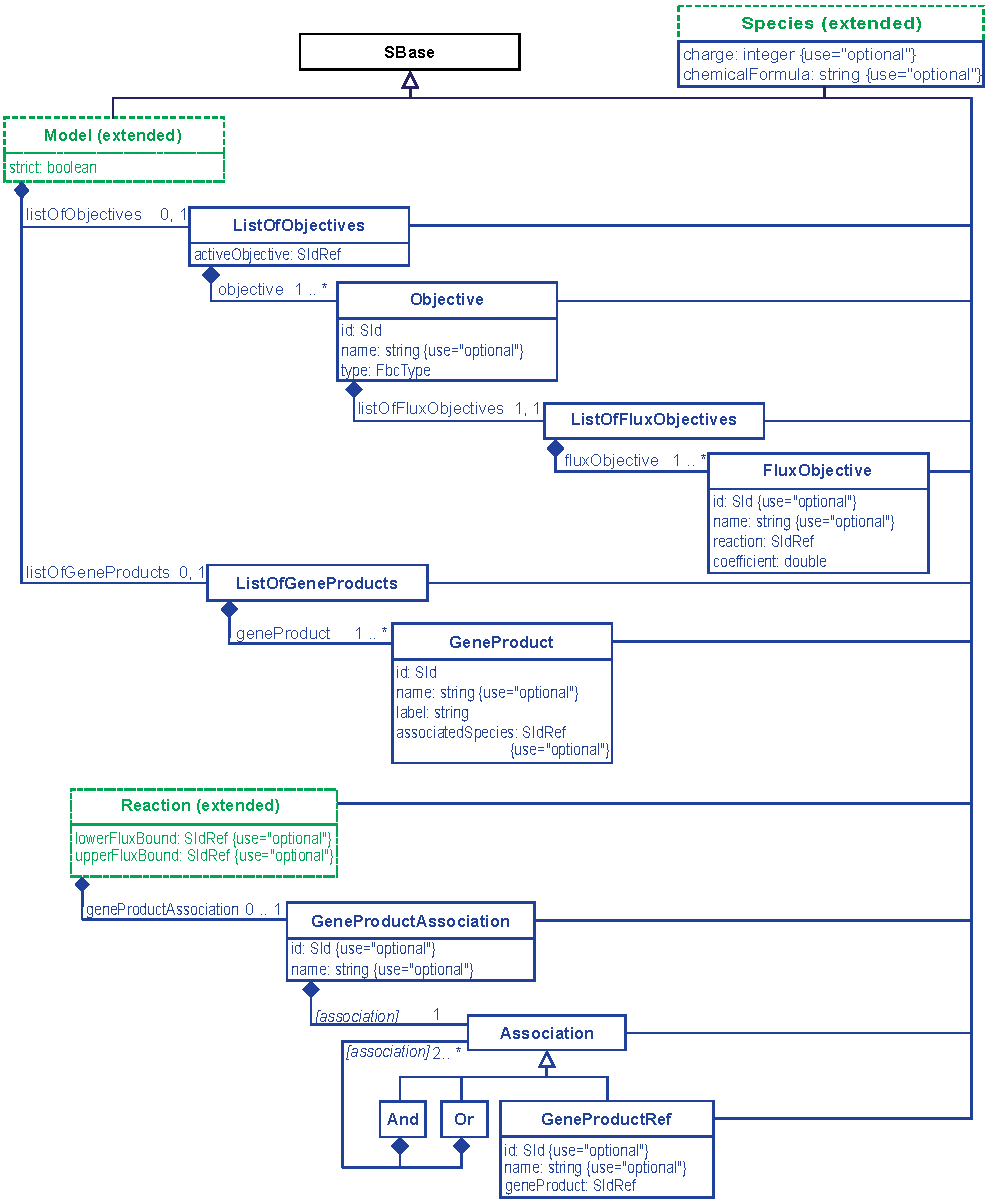
\includegraphics[width=0.85\textwidth]{images/v3harmony_fbc_uml.pdf}\\
  %V3
  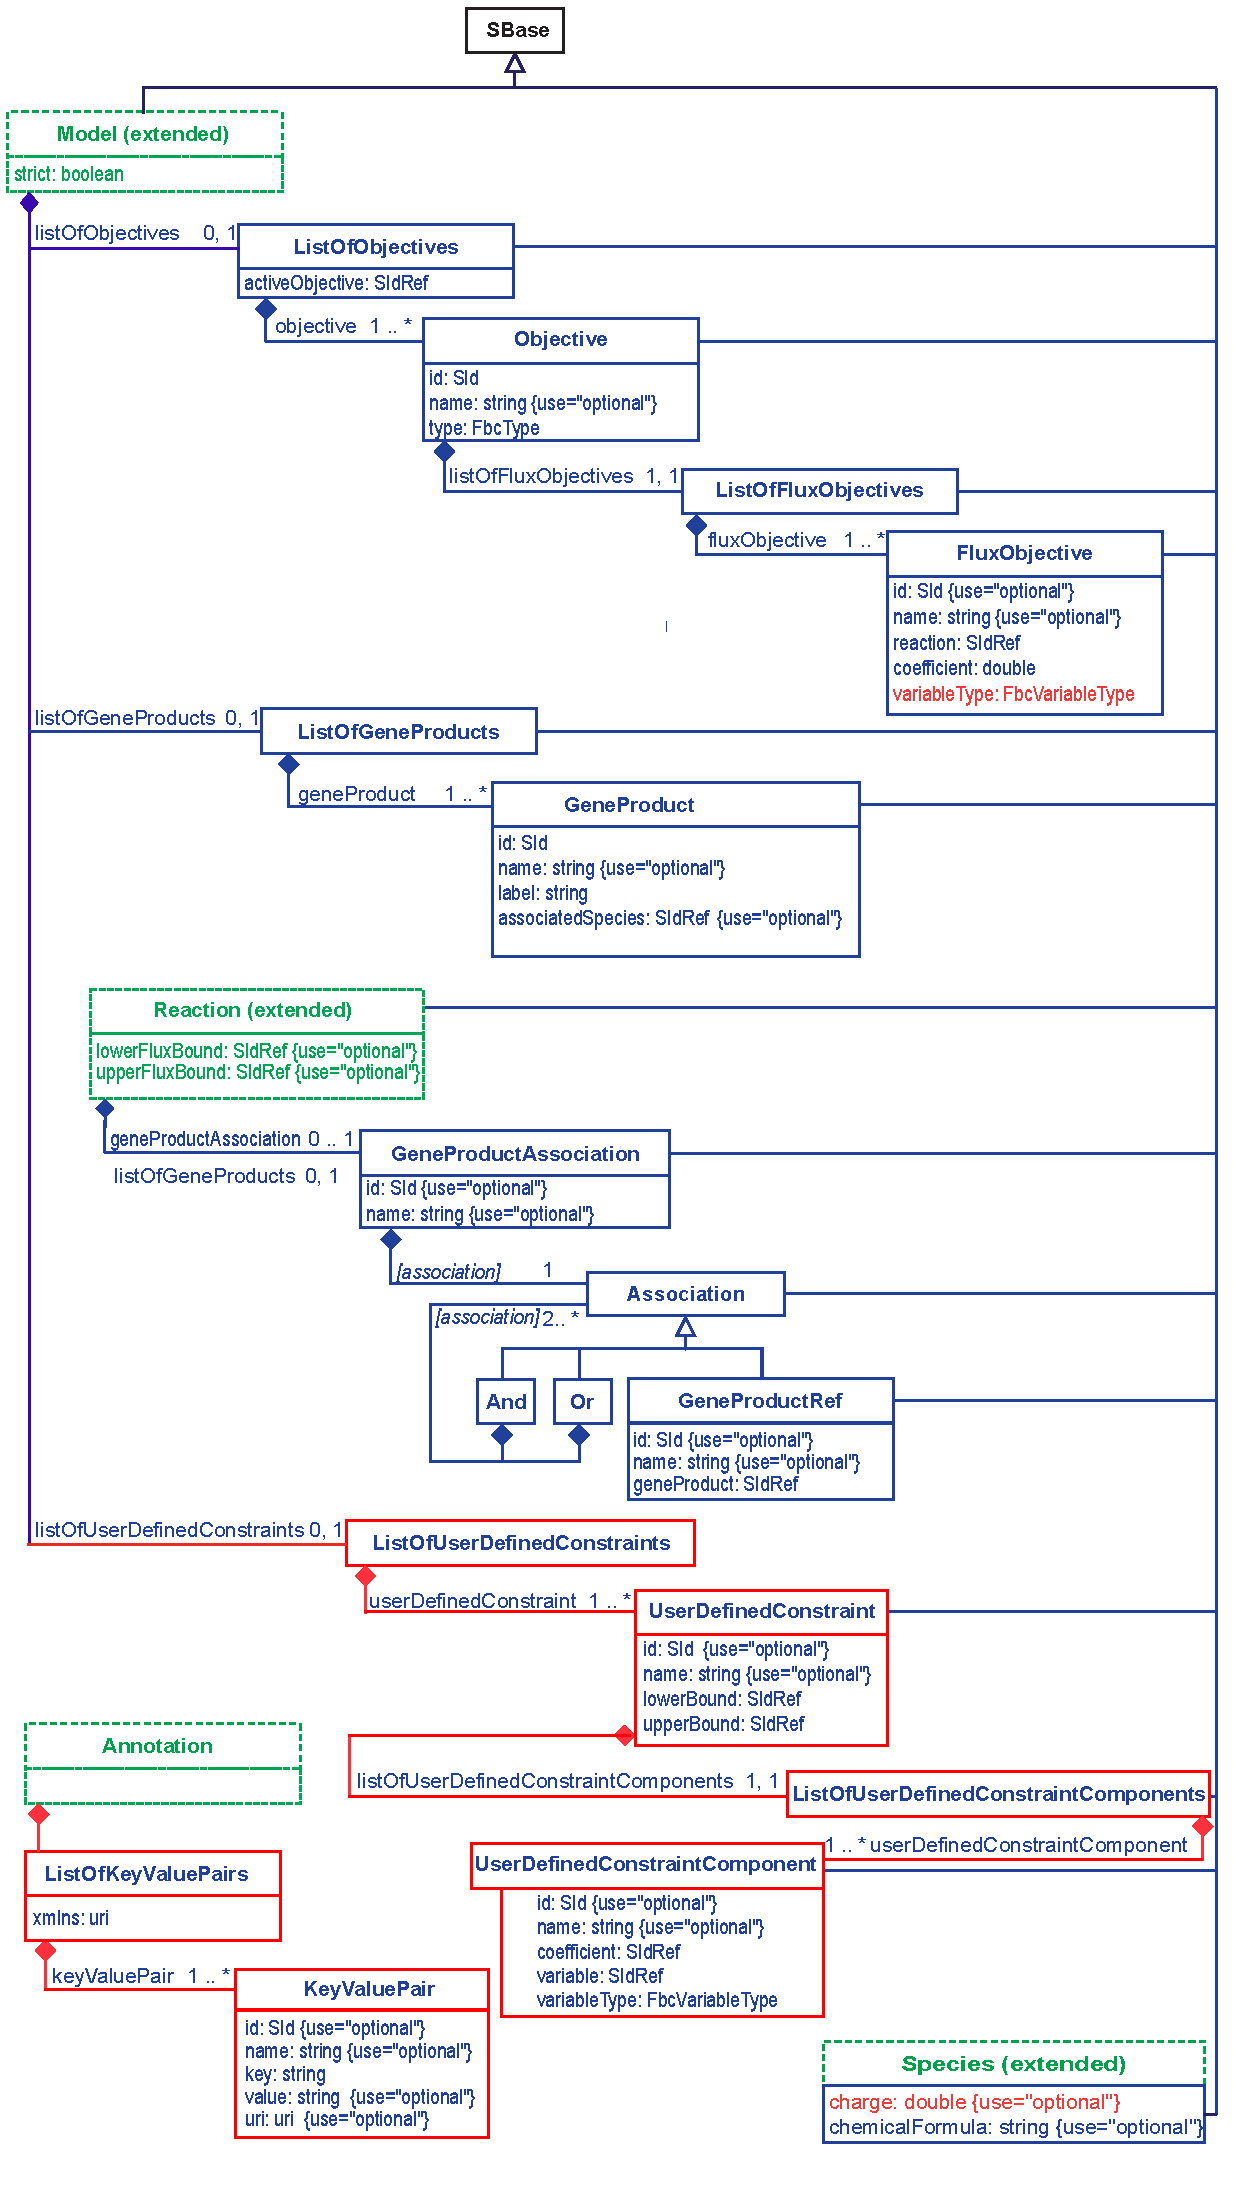
\includegraphics[height=0.85\textheight]{images/fbc_uml_v3.pdf}\\
  \caption{A UML representation of the \FBCPackage. Derived from \SBase, the
	\FBC classes inherit support for constructs such as SBML \Notes and
	\Annotation's. The [association] element name is the name of the class, de-capitalized.  In this case, the possible values are "and", "or", or "geneProductRef". See \ref{conventions} for conventions related to this figure.
	The individual classes are further discussed in the text.}
  \label{fig:fbc_uml}
\end{figure}



\subsection{Primitive data types}
\label{primtypes}

Section~3.1 of the \sbmlthreecore specification defines a number of primitive
data types and also uses a number of XML Schema 1.0 data types~\citep{biron:2000}.
More specifically we make use of \primtype{integer}, \primtype{double},
\primtype{string}, \primtype{SId} and \primtype{SIdRef}. In addition we make
use of a new primitive: the enumeration \primtype{FbcType}, see \ref{fig:fbc_uml}
for the interrelation between
these entities.

\newtxt{The \primtype{SId} type is used as the data type for the identifiers of \Objective (\ref{objective-class}), \FluxObjective (\ref{fluxobjective-class}), \GeneProduct (\ref{geneproduct-class}), \GeneProductAssociation (\ref{geneproductassociation-class}), \GeneProductRef (\ref{geneproductref-class}), \UserDefinedConstraint (\ref{userdefinedconstraint-class}), \UserDefinedConstraintComponent (\ref{userdefinedconstraintcomponent-class}) and \KeyValuePair (\ref{keyvaluepair-class}) classes.}
%
\newtxt{In all cases where the primitive data type \primtype{SId} is used in the \FBCPackage it is used unchanged from its description in \sbmlthreecore. When used as the type of a \token{fbc:id} attribute, that ID is added to the core \primtype{SId} namespace, and must continue to follow those rules for uniqueness: no \token{fbc:id} may duplicate any other \token{fbc:id}, nor the \token{id} of any \Model, \FunctionDefinition, \Compartment, \Species, \Reaction, \SpeciesReference, \ModifierSpeciesReference, \Event, or \Parameter, nor the \token{package:id} of any other SBML Level~3 package element that is also defined as being in the \primtype{SId} namespace.}

In the \FBCPackage the \ListOfObjectives has an attribute of type \primtype{SIdRef} that is used to
refer to an `active' \Objective as does the extended \Reaction class which defines two attributes referring to flux capacity constraints. The \GeneProductRef class declares an attribute of type \primtype{SIdRef} which references a \GeneProduct which itself contains an attribute that can refer to a \Species. \newtxt{Finally, the \UserDefinedConstraint and \UserDefinedConstraintComponent both declare attributes of type \primtype{SIdRef} and a more detailed description of what they refer to can be found in the relevant class descriptions.}

\subsubsection{Type \primtypeNC{FbcType}}
\label{primtype-fbctype}

The \FBCPackage defines a new enumerated type \primtype{FbcType} which represents the optimization sense of the objective function. It can have one of the following two values \val{maximize} or \val{minimize}.

\subsubsection{Type \primtypeNC{FbcVariableType}}
\label{primtype-fbcvariabletype}

\newtxt{The \FBCPackage defines a new enumerated type \primtype{FbcVariableType} which
represents the index of a variable that occurs in either the \FluxObjective or \UserDefinedConstraintComponent. It can have one of two values, \val{linear} or \val{quadratic}.}


\subsection{The extended \class{Model} class}
\label{model-class}
%\label{listoffluxbounds-class}

\newtxt{The \SBML \Model class is extended by adding a mandatory boolean attribute
\token{strict} as well as optional lists: \token{listOfObjectives}, \token{listOfGeneProducts} and \token{listOfUserDefinedConstraints}.} A \Model may contain, at most, one of each of these lists.

\begin{figure}[ht]
  \centering
  % Requires \usepackage{graphicx}
  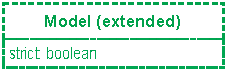
\includegraphics[width=6cm]{images/v3harmony_fbc_model.pdf}\\
  \caption{A UML representation of the extended \SBML \Model class used in
  the \FBCPackage. See \ref{conventions} for conventions related to this
  figure.}
  \label{fig:fbc_uml_model}
\end{figure}


%\begin{deprecated}
%\subsubsection{The \FBC \class{listOfFluxBounds}}
%
%As shown in \ref{fig:fbc_uml} the \ListOfFluxBounds is derived from \SBase
%and inherits the attributes \token{metaid} and \token{sboTerm}, as well as
%the subcomponents for \Annotation and \Notes. \ListOfFluxBounds must contain
%at least one \FluxBound (defined in \ref{fluxbound-class}).
%\end{deprecated}

\paragraph{The attribute \token{strict}}

The mandatory attribute \token{strict}, of type \primtype{boolean}, is used to apply an additional set of restrictions to the model. The \token{strict} attribute ensures that the \FBCPackage can be used to encode legacy FBA models expressible as Linear Programs (LP's) with software that is unable to analyze arbitrary mathematical expressions. In addition it ensures that a `strict' model is fully described and mathematically consistent, for example, by ensuring that all fluxes have a valid upper or lower bound.

\marginpar{\newtxt{How does strict interact with FBC3?}}

This is accomplished by defining a set of restrictions which come into effect if \token{strict} is set to \val{true}:
%
\begin{itemize}
	\item { Each \Reaction in a \Model must define attributes \token{lowerFluxBound} and \token{upperFluxBound} with each pointing to a valid \Parameter object defined in the current \Model.}
	\item {Each \Parameter object referred to by the \Reaction attributes \token{lowerFluxBound} and \token{upperFluxBound} must have their \token{constant} attribute set to \val{true} and its \token{value} attribute set to a \primtype{double} value which may not be \val{NaN}.
	}
	\item { \SpeciesReference elements of {\Reaction}s must have their \token{stoichiometry} attribute set to a \primtype{double} value that is neither \val{NaN} nor \val{-INF} nor \val{INF}. In addition their \token{constant} attribute must be set to \val{true}.
	}
	\item { \InitialAssignment elements may neither target the {\Parameter} elements referenced by the \Reaction attributes \token{lowerFluxBound} and
	        \token{upperFluxBound} nor any \SpeciesReference.
	}
	\item { All defined \FluxObjective elements must have their \token{coefficient} attribute set to a \primtype{double} value that is neither \val{NaN} nor \val{-INF} nor \val{INF}.
	}
	\item { A \Reaction \token{lowerFluxBound} attribute may not point to a \Parameter with a \token{value} of \val{INF}.}
	\item { A \Reaction \token{upperFluxBound} attribute may not point to a \Parameter with a \token{value} of \val{-INF}.}
    \item {For all reactions, the value of a \token{lowerFluxBound} must be less than or equal to the value of the \token{upperFluxBound}.}

\end{itemize}
%
While it is not compulsory for a `strict' \FBC model to define an \Objective, doing so does does allow it to be formulated as an LP and optimized, however, this decision is left to the modeler. Note that all other properties of the elements referred to in this list are as specified in the relevant \sbmlthreecore and \FBC specifications.

Alternatively, if the value of the \token{strict} attribute is \val{false} then none of these restrictions apply and the model creator can choose to define \FBC models that are not necessarily encodable as a LP. For example, if \token{strict} is \val{false} the \InitialAssignment construct may be used to set any valid numerical entity, including \Parameter values and stoichiometric coefficients, with any \primtype{double}. In addition, \Parameter elements are no longer required to be flagged as `constant' thus allowing for an \FBC model's use in alternative, hybrid modeling strategies.

\subsubsection{The \FBC \class{listOfObjectives}}
\label{listofobjectives-class}
As shown in \ref{fig:fbc_uml} the \ListOfObjectives is derived from \SBase
and inherits the attributes \token{metaid} and \token{sboTerm}, as well as
the subcomponents for \Annotation and \Notes. Unlike most other \SBML
\textsf{\textbf{ListOf\rule{0.15in}{0.5pt}}} classes, \ListOfObjectives
introduces an additional required attribute \token{activeObjective}. The
\ListOfObjectives must contain at least one \Objective (defined in
\ref{objective-class}).

\paragraph{The \token{activeObjective} attribute}
\label{activeObjective-attribute}

This attribute is of type \primtype{SIdRef} and can only refer to the
\token{id} of an existing \Objective. This required attribute exists
so that when multiple \Objective's are included in a single model, the
model will always be well described i.e., there is a single, primary
objective function which defines a single optimum and its associated
solution space.

\subsubsection{The \FBC \class{listOfGeneProducts}}
\label{listofgeneproducts-class}

As shown in \ref{fig:fbc_uml} the \ListOfGeneProducts is derived from \SBase
and inherits the attributes \token{metaid} and \token{sboTerm}, as well as
the subcomponents for \Annotation and \Notes. The \ListOfGeneProducts must
contain at least one \GeneProduct (defined in \ref{geneproduct-class}).

\subsubsection{The \FBC \class{listOfUserDefinedConstraints}}
\label{listofuserdefinedconstraints-class}

\newtxt{As shown in \ref{fig:fbc_uml} the \ListOfUserDefinedConstraints is derived from \SBase and inherits the attributes \token{metaid} and \token{sboTerm}, as well as the subcomponents for \Annotation and \Notes. The \ListOfUserDefinedConstraints must contain at least one \UserDefinedConstraint (defined in \ref{userdefinedconstraint-class}).}

\subsubsection{A note on units}
\label{fbcunits}
The main unit definitions that should be considered when using the \FBCPackage
are the global model definitions of ``extent''  and ``time'' as all \FBC flux
related classes (i.e., %\FluxBound and
\FluxObjective implicitly attains the same
unit as the \Reaction that they reference). More details on units can be found
in their respective class definitions.

\subsection{The extended \class{Species} class}
\label{species-class}

The \FBCPackage extends the \sbmlthreecore \Species class with the addition
of two attributes \token{charge} and \token{chemicalFormula}.
%
\begin{figure}[h]
  \centering
  % Requires \usepackage{graphicx}
  %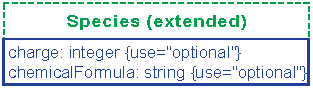
\includegraphics[width=6cm]{images/v2harmony_fbc_species.pdf}\\
  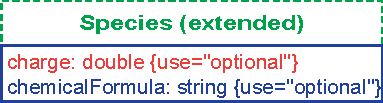
\includegraphics[width=6cm]{images/v3harmony_fbc_species.pdf}\\
  \caption{A UML representation of the extended \SBML \Species class used in
  the \FBCPackage. See \ref{conventions} for conventions related to this
  figure.}
  \label{fig:fbc_uml_species}
\end{figure}


%\paragraph{The \token{charge} attribute}
%The optional attribute \token{charge} which contains a signed
%\primtype{integer} referring to the \Species object's charge and is
%defined as it was in the \SBML Level 2 Version 1 specification
%: \textit{``The optional field charge takes an integer indicating
%the charge on the species (in terms of electrons, not the SI unit coulombs).''}
%
%\paragraph{The \token{chemicalFormula} attribute}
%\label{chemicalFormula-attribute}
%The optional attribute \token{chemicalFormula} containing a
%\primtype{string} that represents the \Species objects elemental
%composition.
%%
%\exampleFile{examples/ex_spec_l3.txt}
%%
%While there are many ways of referring to an elemental composition the purpose
%of the \token{chemicalFormula} attribute is to allow reaction balancing and
%validation which is particularly important in constraint-based models.
%
%The format of \token{chemicalFormula} must consist only of atomic names (as in
%the Periodic Table) or user defined compounds either of which take the form of
%a single capital letter followed by zero or more lowercase letters. Where there
%is more than a single atom present, this is indicated with an integer. With
%regards to order (and enhance inter-operability) it is recommended to use the
%Hill system order \citep{hillsystem, hillwikipedia}.
%
%%
%\begin{table}[h!]
%  %\centering
%  H2O4S\qquad C2H5Br\qquad BrH\\
%  C10H12N5O13P3\qquad CH3I\\
%  \caption{Examples of chemical formulas written using the Hill System. As
%	described in \ref{chemicalFormula-attribute}}\label{table:hill}
%\end{table}
%%
%Using this notation the number of carbon atoms in a molecule is indicated
%first, followed by the number of hydrogen atoms and then the number of all
%other chemical elements in alphabetical order. When the formula contains no
%carbon; all elements, including hydrogen, are listed alphabetically.

\paragraph{The \token{charge} attribute}

\newtxt{The optional attribute charge contains a signed double referring to the Species object’s charge (in terms of electrons, not the SI unit coulombs). Note, that unlike FBC versions one and two a \Species may, for the purposes of charge, be interpreted as a pseudoisomer or aggregate molecule and may assume a non-integer value. Non-integer charges should be used with caution as their use may have unintended side-effects, for example, with respect to the accuracy of reaction balancing.}

\paragraph{The \token{chemicalFormula} attribute}
\label{chemicalFormula-attribute}

The optional attribute \token{chemicalFormula} containing a \primtype{string} that represents the \Species objects elemental composition.

\newtxt{While there are many ways of referring to an elemental composition, the purpose of the \token{chemicalFormula} attribute is to enable reaction balancing and validation, something of particular importance in constraint-based models.}

\newtxt{The format of the \token{chemicalFormula} should, whenever possible, consist only of atomic names
(as in the Periodic Table). Similarly, for enhanced inter-operability, the element order should be arranged according to the Hill system (see \ref{table:hill2})} \citep{hillsystem, hillwikipedia}.
%
\begin{table}[h!]
  \begin{tabular}{ccc}
    % after \\: \hline or \cline{col1-col2} \cline{col3-col4} ...
     $H_{2}O_{4}S$ & $C_{2}H_{5}Br$ & $BrH$ \\
     $C_{10}H_{12}N_{5}O_{13}P_{3}$ & $CH_{3}I$ & $CH_{4}$  \\
  \end{tabular}
  \caption{Examples of chemical formulas written using the Hill System. As
	described in \ref{chemicalFormula-attribute}}\label{table:hill2}
\end{table}
%
\newtxt{Using this notation the number of carbon atoms in a molecule is indicated first, followed by the number of hydrogen atoms and then the number of all other chemical elements in alphabetical order. When the formula contains no carbon; all elements, including hydrogen, are listed alphabetically. Where there is more than a single atom present, this is indicated with an integer that follows the element symbol.}

\exampleFile{examples/ex-v3-species.txt}
%
\newtxt{However, in certain situations, it may become necessary to use a generic symbol to represent an undefined or generic component of a user-defined compound. Generic components can only be specified as the symbols \textsf{R} or \textsf{X}.}
%
\begin{table}[h!]
  \begin{tabular}{ccc}
    % after \\: \hline or \cline{col1-col2} \cline{col3-col4} ...
     $RCONH_{2}$ & $COX$ & $C_{2}H_{4}O_{2}(CH_{2})_{n}$ \\
  \end{tabular}
  \caption{Examples of chemical formulas written using the allowed non-Hill symbols described in \ref{chemicalFormula-attribute}.}\label{table:non-hill}
\end{table}
%
\newtxt{Furthermore, the undefined parenthesised group index $(\ldots)_n$ may also be used to indicate an arbitrary repetition of a chemical group. Note that a parenthesized group may only be followed by the subscript $n$. Integer values, for example, $(\ldots)_2$ and expressions such as $(\ldots)_{n-1}$ are considered invalid chemical formula.}

\newtxt{Please note, the use of \textsf{R}, \textsf{X} and $(\ldots)_n$ is not generally advised, as any \Reaction in which such a \Species occurs cannot necessarily be balanced and may lead to the construction of an invalid model. To highlight this potential problem, any \token{chemicalFormula} that contains any of the aforementioned, non-Hill compatible symbols will raise a `best practices' warning on model validation.}

\subsection{The \FBC \class{GeneProduct} class}
\label{geneproduct-class}
\GeneProduct is a new \FBC class derived from \SBML \SBase that inherits
\token{metaid} and \token{sboTerm}, as well as the subcomponents for
\Annotation and \Notes. The purpose of this class is to define a single gene
product. It implements two required attributes \token{id} and \token{label} as
well as two optional attributes \token{name} and \token{associatedSpecies}.

\begin{figure}[h]
  \centering
  % Requires \usepackage{graphicx}
  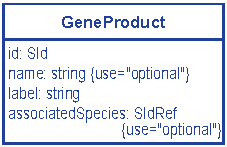
\includegraphics[width=5cm]{images/v2harmony_fbc_geneproduct.pdf}\\
  \caption{A UML representation of the \FBCPackage \GeneProduct class. For a complete description see \ref{fig:fbc_uml} as well as \ref{conventions} for conventions related to this figure.}
  \label{fig:fbc_uml_geneproduct}
\end{figure}

\paragraph{The \token{id} and \token{name} attributes}
A \GeneProduct has a required attribute \token{id} of type \primtype{SId}
and an optional attribute \token{name} of type \primtype{string}. The
unique \token{id} attribute is required to enable a \GeneProduct to be
referenced from a \GeneProductRef used in a \GeneProductAssociation.

\paragraph{The \token{label} attribute}
The primary purpose of a \GeneProduct is to uniquely reference a gene or
implied gene product. As there is, currently, no restriction on the format of these these references they cannot be assumed to conform to an \SBML \primtype{SId} syntax. Therefore the \FBCPackage defines the required attribute \token{label}, of type \primtype{string}, for this purpose.

%as seen in the example shown in \ref{intro-ga}
% % FB: taken out the sentence, as it does not add to the text
% As can be seen from the following examples, taken from existing models:
% \verb+Rv0649+, \verb+3074.1+ and \verb+CRv4_Au5.s2.g9153.t1+ there is
% currently no defined format for this gene identifier.
While ideally some form of restriction could, in principle, be placed on the value of \token{label}, at this point in time it is only possible to suggest that this attribute's value should conform to the definition of an
\primtype{SId}. For example, consider an existing GPR annotation, as encountered in legacy \SBML Level 2 encoded models:
\begin{verbatim}
 <p>GENE_ASSOCIATION: (Rv0649)</p>
\end{verbatim}
%
this can now be formally (and unambiguously) encoded as:
%
\exampleFile{examples/v2harmony-spec-example1-gene.txt}

Furthermore, it is a highly recommended `best practice' that a \GeneProduct be annotated using the inherited MIRIAM compliant \SBML \Annotation mechanism. Doing so will help reduce the dependence and ambiguity of using an overloaded, semantically meaningful \token{label} attribute and enhance interoperability. For an example of this approach see \ref{best-practices-cobraV2}.

\paragraph{The \token{associatedSpecies} attribute}
A \GeneProduct may, optionally, refer to a \Species so as to provide compatibility with the Manchester style encoding of gene-protein associations. In this case the attribute \token{associatedSpecies} is of type \primtype{SIdRef} and, if defined, must point to an existing \Species in the model.

%\begin{deprecated}
%\subsection{The \FBC \class{FluxBound} class}
%\label{fluxbound-class}
%
%\FluxBound is a new \FBC class derived from \SBML \SBase that inherits
%\token{metaid} and \token{sboTerm}, as well as the subcomponents for
%\Annotation and \Notes. The purpose of this class is to hold a single
%(in)equality that provides the maximum or minimum value that a reaction flux
%can obtain at steady state. It implements three attributes.
%
%Starting with Version~2 of the Flux Balance Constraints package the
%\FluxBound construct is deprecated. This is done to ease adoption and ensure that
%not all tools have to immediately implement support for changing flux bounds the
%attributes may also refer to the an existing \FluxBound in the model. However,
%that construct is deprecated and will be removed in a future version of this
%package.
%
%
%\begin{figure}[h!]
  %\centering
  %% Requires \usepackage{graphicx}
  %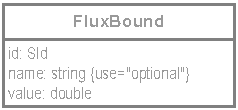
\includegraphics[width=5cm]{images/v2harmony_fbc_fluxbound.pdf}\\
  %\caption{A UML representation of the \FBCPackage \FluxBound class. See
  %\ref{conventions} for conventions related to this figure.}
  %\label{fig:fbc_uml_fbnd}
%\end{figure}
%
%\paragraph{The \token{id} and \token{name} attributes}
%A \FluxBound has the required attributes: \token{id} an attribute of type
%\primtype{SId} and an optional attribute \token{name} an attribute of type
%\primtype{string}.
%
%\paragraph{The \token{value} attribute}
%The \token{value} attribute holds a \primtype{double} value representing the
%numerical value of the flux bound. This may include an explicitly defined
%$\pm\infty$ encoded as a value, e.g., \val{INF}.
%
%For an example of the how the \FluxBound relates to the description of the
%underlying mathematical model please see \ref{examples1:fluxbound}.
%
%\paragraph{Units}
%The \token{value} defined by the \FluxBound has the units of the \token{reaction}
%that it refers to i.e.,~the globally defined unit of ``extent per time.''
%
%\paragraph{Reactions with undefined flux bounds}
%In the spirit of \sbmlthreecore the \FBCPackage does not define any default
%values for any element. However, in the case of a reaction with no defined
%flux bounds it is possible to infer this information from the reaction
%reversibility. In this case: irreversible reactions should be considered to
%be positive, $0 <= J <= \infty$ and reversible ones free/unbound,
%$-\infty <= J <= \infty$.
%
%Similarly, there is also the potential for a bound to ``seemingly'' conflict
%with the reaction that it bounds' reversibility, e.g., a reaction is
%irreversible but has bounds $-\infty <= J <= \infty$. In the context of
%this package, flux bounds should be considered authoritative. This follows
%from the fact that a \FluxBound can enforce an irreversible reaction, by
%restricting the flux ($0 <= J <= \infty$), as well as a reversible
%reaction ($-\infty <= J <= \infty$). It is left to the software
%implementation to deal with any obvious inconsistencies.
%
%\end{deprecated}

%\newpage

\subsection{The \FBC \class{Objective} class}
\label{objective-class}
\label{listoffluxobjectives-class}

The \FBC \Objective class is derived from \SBML \SBase and inherits
\token{metaid} and \token{sboTerm}, as well as the subcomponents for
\Annotation and \Notes. An integral component in a complete description
of a steady-state model is the so-called `objective function' which generally
consist of a linear combination of model variables (fluxes) and a sense
(direction). In the \FBC package this concept is succinctly captured in the
\Objective class.

\paragraph{The \token{id} and \token{name} attributes}
An \Objective has a required attribute \token{id} of type
\primtype{SId} and an optional attribute \token{name} of type \primtype{string}.

\paragraph{The \token{type} attribute}
The required \token{type} attribute contains an \primtype{FbcType} type
which represents the sense of the optimality constraint and can take one of
two values:
\begin{eqnarray*}
% I'm using \mapsto until I can find the proper symbol - bgoli
\label{obj-type-enum}
 \nonumber
  maximize & \mapsto & \textrm{``}\mathtt{maximize}\textrm{''}\\
  minimize & \mapsto & \textrm{``}\mathtt{minimize}\textrm{''}
\end{eqnarray*}

\paragraph{The \token{listOfFluxObjectives} element}
The element \token{listOfFluxObjectives} which contains a
\ListOfFluxObjectives is derived from and functions like a typical \SBML
\textsf{\textbf{ListOf\rule{0.15in}{0.5pt}}} class with the restriction that it
must contain one or more elements of type \FluxObjective (see \ref{fluxobjective-class}).
This implies that if an \Objective is defined there should be at least
one \FluxObjective contained in a \ListOfFluxObjectives.
% bgoli: to me this makes sense but are there other examples of this in SBML or is everything always optional

\begin{figure}[ht]
  \centering
  % Requires \usepackage{graphicx}
  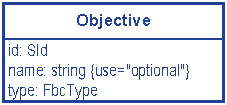
\includegraphics[width=5cm]{images/v2harmony_fbc_objective.pdf}\\
  \caption{A UML representation of the \FBCPackage \Objective class. For a complete description see \ref{fig:fbc_uml} as well as \ref{conventions} for conventions related to this figure.}
  \label{fig:fbc_uml_obj}
\end{figure}

\pagebreak
\paragraph{Encoding the \Objective}
The \FBCPackage allows for the definition of multiple model objectives with
one being designated as active (see \ref{objective-class}) as illustrated in
this example:
%
\exampleFile{examples/ex_objf_fbc.txt}
%
Note how both \Objective instances differ in \token{type} and each contains
different set of \class{FluxObjectives} (see \ref{fluxobjective-class}).
For an example of how the \Objective relates to the description of the
underlying mathematical model please see \ref{examples1:objfunc}.

%\subsection{The \FBC \class{FluxObjective} class}
%\label{fluxobjective-class}
%
%The \FBC \FluxObjective class is derived from \SBML \SBase and inherits
%\token{metaid} and \token{sboTerm}, as well as the subcomponents for
%\Annotation and \Notes.
%
%The \FluxObjective class is a relatively simple container for a model
%variable weighted by a signed linear coefficient.
%
%%
%\begin{figure}[ht]
%  \centering
%  % Requires \usepackage{graphicx}
%  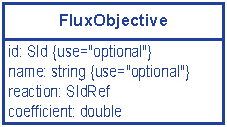
\includegraphics[width=5cm]{images/v2harmony_fbc_fluxobjective.pdf}\\
%  \caption{A UML representation of the \FBCPackage \FluxObjective class. For a complete description see \ref{fig:fbc_uml} as well as \ref{conventions} for conventions related to this figure.}
%  \label{fig:fbc_uml_fobj}
%\end{figure}
%
%\paragraph{The \token{id} and \token{name} attributes}
%A \FluxObjective has two optional attributes: \token{id} an attribute of
%type \primtype{SId} and \token{name} an attribute of type \primtype{string}.
%
%\paragraph{The \token{reaction} and \token{coefficient} attributes}
%The required \token{reaction} is of type \primtype{SIdRef} and is restricted
%to refer only to a \Reaction while the \token{coefficient} attribute
%holds a \primtype{double} referring to the coefficient that this \FluxObjective
%takes in the enclosing \Objective. For example the objective
%\texttt{ Maximize: 1 R1 + 2 R2} would be encoded as
%%
%\exampleFile{examples/ex_fluxobj_fbc.txt}
%
%\paragraph{Units}
%As described above the \FluxObjective defined here as $n\cdot J$ where
%the \token{coefficient} ($n$) is dimensionless and the \token{value} ($J$)
%takes the units of the \token{reaction} flux i.e.,~``extent per time''.
%Therefore, the \FluxObjective ($n\cdot J$)  has the unit ``extent per time''
%where the units of reaction ``extent'' and ``time'' are defined globally.

\subsection{The \FBC \class{FluxObjective} class}
\label{fluxobjective-class}

The \FBC \FluxObjective class is derived from \SBML \SBase and inherits \token{metaid} and \token{sboTerm}, as well as the subcomponents for \Annotation and \Notes.
%
\newtxt{The FluxObjective class is a relatively simple container for a model variable weighted by a signed numerical coefficient. The model variable is defined as being either a `linear' or `quadratic' variable.}
%
\begin{figure}[ht]
  \centering
  % Requires \usepackage{graphicx}
  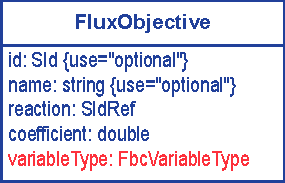
\includegraphics[width=6cm]{images/fbc_v3_uml_fobj.pdf}\\
  \caption{A UML representation of the \FBCPackage \FluxObjective class. For a complete description see \ref{fig:fbc_uml} as well as \ref{conventions} for conventions related to this figure.}
  \label{fig:fbc_uml_userdefinedconstraint}
\end{figure}
%
% I don't thing this is needed
%\newtxt{The \FluxObjective class is a relatively simple container for a model variable that can be defined as the variable type `linear' or `quadratic' and weighted by a signed linear coefficient.}
%
\paragraph{The \token{id} and \token{name} attributes}
A \FluxObjective has two optional attributes: \token{id} an attribute of
type \primtype{SId} and \token{name} an attribute of type \primtype{string}.

\paragraph{The \token{reaction} and \token{coefficient} attributes}
The required \token{reaction} is of type \primtype{SIdRef} and is restricted
to refer only to a \Reaction while the \token{coefficient} attribute
holds a \primtype{double} referring to the coefficient that this \FluxObjective
takes in the enclosing \Objective expression.

\newtxt{\paragraph{The \token{variableType} attribute}
The required \token{variableType} attribute contains a \primtype{FbcVariableType} that
represents the index to which a variable is raised in a \FluxObjective. For example, where $J$ represents a steady-state flux the \primtype{FbcVariableType} defines either a \val{linear}, $J^1$ or \val{quadratic}, $J^2$ term.}

\paragraph{Two examples of objective functions encoded in \SBML}
\newtxt{A common linear objective function (expressed in LP format):} \verb"Maximize: 1 R1"
%
\exampleFile{examples/ex-v3-fluxobjective-linear.txt}
%
\newtxt{An advanced objective function with both a linear and quadratic term (expressed in LP format):} \verb"Minimize: 1 R1 + [4 R2^2]/2"
%
\exampleFile{examples/ex-v3-fluxobjective.txt}

\paragraph{Units}
As described above the linear \FluxObjective defined here as $n\cdot J$ where
the \token{coefficient} ($n$) is dimensionless and the \token{value} ($J$)
takes the units of the \token{reaction} flux i.e.,~``extent per time''.
\newtxt{Therefore, the \token{linear} \FluxObjective, ($n\cdot J$)  has the unit $\frac{extent}{time}$ where the units of reaction ``extent'' and ``time'' are defined globally. Analogously, in the case of a \token{quadratic} \FluxObjective, $n\cdot J^{2}$ this would be $\frac{extent^{2}}{time^{2}}$}.


% -*- TeX-master: "main"; fill-column: 72 -*-

%\subsection{Encoding Gene Protein Associations in SBML}

%This specification drafted by \emph{Brett G. Olivier} and \emph{Frank T. Bergmann} (2013) with contributions by members of the \emph{FBC working group} as well as \emph{FBC} and \emph{SBML} communities. It builds on and supersedes the proposal included in \ref{future} of the \FBCPackage version 1 specification and as such implemented as an annotation in \textsf{libSBML}.

%\subsection{ Introduction and motivation }
%\label{intro-ga}

%\subsection{The extended \class{Model} class}
%\label{listofgeneproteinassociations-class}
%
%\subsubsection{The \FBC \class{listOfGeneProteinAssociations}}
%
%The \ListOfGeneProteinAssociations extends \sbmlthreecore, is derived from \SBase and inherits the attributes \token{metaid} and \token{sboTerm} as well as the subcomponents for \Annotation and \Notes (as shown in \ref{fig:fbc_uml_ga_all}). If defined \ListOfGeneProteinAssociations must contain at least one \GeneProductAssociation (as defined below in \ref{geneproductassociation-class}).
%
%\subsection{The extended \class{Species} class}
%\label{species-class-ga}
%
%The \FBCPackage \textsf{Gene Association Proposal} (this document) extends the \sbmlthreecore \Species class (in addition to \token{charge} and \token{chemicalFormula}) with the addition of an attribute \token{isGene}.
%%
%\begin{figure}[h!]
%  \centering
%  % Requires \usepackage{graphicx}
%  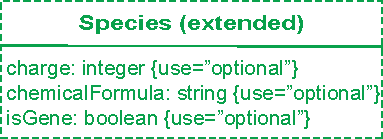
\includegraphics[width=6cm]{images/fbc_uml_species-v2.pdf}\\
%  \caption{A UML representation of the extended \SBML \Species class used in
%  the \FBCPackage. See \ref{conventions} for conventions related to this
%  figure.}
%  \label{fig:fbc_uml_species_ga}
%\end{figure}
%
%\paragraph{The \token{isGene} attribute}
%The optional attribute \token{isGene} contains a \primtype{boolean} referring to the fact that the \Species is not a metabolite that should be included in the reaction network but rather represents a \GeneProductRef product that participates in an \Association. In addition for a \Species where \verb+isGene="true"+ there should be at least one \GeneProductRef that refers to it via its \token{species} attribute (for more details see \ref{geneproductref-class}).
%%
%\exampleFile{examples/ex_spec_l3_v2.txt}

%
%\subsubsection{The \FBC \class{listOfGeneProteinAssociations}}
%
%The \ListOfGeneProteinAssociations extends \sbmlthreecore, is derived from \SBase and inherits the attributes \token{metaid} and \token{sboTerm} as well as the subcomponents for \Annotation and \Notes (as shown in \ref{fig:fbc_uml_ga_all}). If defined \ListOfGeneProteinAssociations must contain at

%\begin{figure}[h!]
%  \centering
%  % Requires \usepackage{graphicx}
%  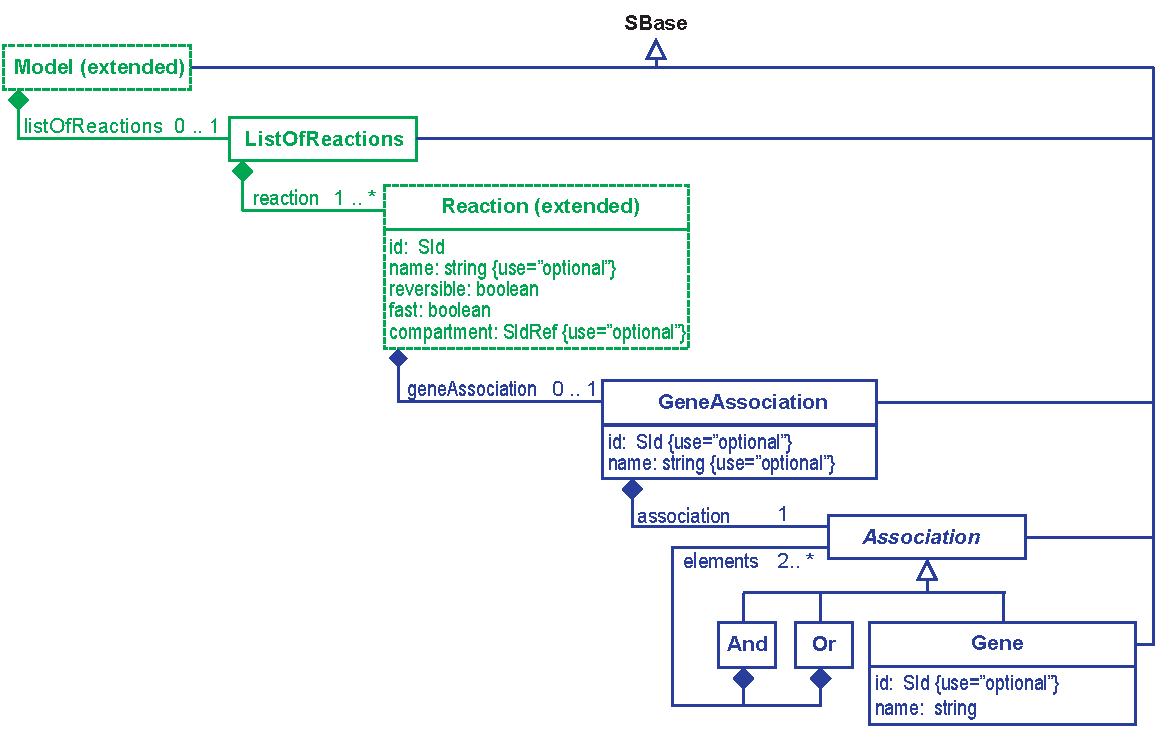
\includegraphics[width=\textwidth]{images/fbc_uml_ga_all2.pdf}\\
%  \caption{A UML representation of the \FBCPackage. Derived from \SBase, the \FBC classes inherit support for constructs such as SBML \Notes and \Annotation's. See \ref{conventions} for conventions related to this figure. The individual classes are further discussed in the text.}
%  \label{fig:fbc_uml_ga_all}
%\end{figure}

\subsection{The extended \class{Reaction} class}
\label{reaction-class-ga}

The \FBCPackage extends the \sbmlthreecore \Reaction class with the addition of
a new optional element \GeneProductAssociation as well as two optional attributes
\token{lowerFluxBound} and \\
\token{upperFluxBound}.

\begin{figure}[h]
  \centering
  % Requires \usepackage{graphicx}
  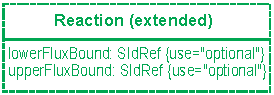
\includegraphics[width=6cm]{images/v2harmony_fbc_reaction.pdf}\\
  \caption{A UML representation of the extended \SBML \Reaction class used in
  the \FBCPackage. For a complete description see \ref{fig:fbc_uml} as well as \ref{conventions} for conventions related to this figure.}
  \label{fig:fbc_uml_reaction}
\end{figure}

\paragraph{The attributes \token{lowerFluxBound} and \token{upperFluxBound}}
The optional attributes \token{lowerFluxBound} and \token{upperFluxBound} of type \primtype{SIdRef} are used to specify the lower and upper flux bounds for a \Reaction flux.

The attributes must refer to an existing \Parameter in the model and in the case that equal bounds are required for a reaction, both attributes should point to the same \Parameter. The \FBCPackage specifies Systems Biology Ontology (SBO) terms that can be used to define the character of such a \Parameter, please see the appendix describing SBO for more details.

Using a \Parameter in this way makes it possible for other SBML elements to interact with these parameters depending on the value of the \token{fbc:\-strict} attribute of the \Model (see also \sec{model-class}).

For example, if the value of the \token{strict} attribute is \val{false}, even in the case of a constant \Parameter (i.e. SBML parameters that have their \token{constant} attribute set to \val{true}) the value of a flux bound's value could be calculated using an \InitialAssignment. Should the parameter not be constant, then its value can be additionally updated by all \sbmlthreecore constructs (for example \EventAssignment, \AssignmentRule and \AlgebraicRule). However none of the aforementioned applies when the \token{strict} attribute is set to \val{true}.

%\begin{deprecated}
%{
%To ease adoption and ensure that not all tools have to immediately implement
%support for changing flux bounds the attributes may also refer to the an existing
%\FluxBound in the model. However, that construct is deprecated and will be removed
%in a future version of this package.
%}
%\end{deprecated}

\paragraph{Encoding the flux bounds}
\newtxt{To generate a list of (in)equalities for each reaction from the parameters reference in \texttt{upperFluxBound} and \texttt{lowerFluxBounds}, one must first resolve the reference to the underlying \Parameter. If both bounds refer to the same element they generate an equality, as shown in Equation~1. Alternatively, when two elements are referenced as flux bounds, two inequalities are generated, as shown in Equations 2 and 3:
%
\begin{eqnarray}
% \nonumber to remove numbering (before each equation)
  \token{reaction} &=& \token{value} \\
  \token{reaction} &\geq& \token{lowerFluxBound value} \\
  \token{reaction} &\leq& \token{upperFluxBound value}
\end{eqnarray}
}

In SBML Level~3 Version~1 with \FBC Version~3 this is encoded as:
%
\exampleFile{examples/v2harmony-ex_fb_fbc.txt}

%\begin{deprecated}
%
%In case no evaluation of \InitialAssignment, \EventAssignment, \AssignmentRule,
%and \AlgebraicRule is desired, it is possible to continue using the \FluxBound
%construct using the same scheme:
%
%% don't include example
%%\exampleFile{examples/v2harmony-ex_fb_fbc_dep.txt}
%
%\end{deprecated}

%


%This example illustrates two things: the encoding of $\infty$ and that care
%should be used when selecting inequalities such as \val{less} or
%\val{greater}. While mathematically there is a difference, this difference
%is only practically relevant when working with rational arithmetic
%(solvers).
%

%


\subsection{The \FBC \class{GeneProductAssociation} class}
\label{geneproductassociation-class}

The \FBCPackage defines a \GeneProductAssociation class that derives
from \SBase and inherits the attributes \token{metaid} and \token{sboTerm}
as well as the subcomponents for \Annotation and \Notes. As shown in
\ref{fig:fbc_uml} the \GeneProductAssociation class extends \Reaction with
one or more genes (or gene products). Where more than one gene (or gene product) is present in an association they are written as logical expressions and thereby related to one another using logical `and' and `or' operators.

\paragraph{The \token{id} and \token{name} attributes}
A \GeneProductAssociation has two optional attributes: \token{id} an attribute of
type \primtype{SId} and \token{name} an attribute of type \primtype{string}.

%\paragraph{The \token{reaction} attribute}
%The required \token{reaction} attribute of type \primtype{SIdRef}. This attribute must refer to a \Reaction element defined within the enclosing model.

\paragraph{The \token{association} element}
Each \GeneProductAssociation contains a single \Association, however, as
described in \ref{association-class} an \Association is an abstract class
that implies that an \token{association} will always contain an instance
of one of its sub-classes: \GeneAnd, \GeneOr or \GeneProductRef.
%
\begin{figure}[h!]
  \centering
  % Requires \usepackage{graphicx}
  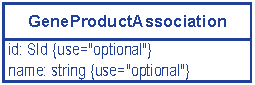
\includegraphics[width=5cm]{images/v2harmony_fbc_geneproductassociation.pdf}\\
  \caption{A UML representation of the \FBCPackage \GeneProductAssociation class.
	For a complete description see \ref{fig:fbc_uml} as well as \ref{conventions} for conventions related to this figure.}
  \label{fig:fbc_uml_ga}
\end{figure}

\paragraph{Encoding the \GeneProductAssociation}
As described in \ref{geneproductassociation-class}, the \GeneProductAssociation
is simply a container that contains one of three types of \Association either
holding a single \GeneProductRef or two or more \Association elements in an
\GeneAnd or \GeneOr relationship. For example, the following typical
gene--protein association expression from the BiGG database \emph{E.~coli}
reconstruction (iJR904; \citealt{ijr904, bigg})
%
\begin{verbatim}
 ((B3670 and B3671) or (B0077 and B0078) or (B3768 and B3769 and B3767))
\end{verbatim}
%
can now be encoded as:
%
\exampleFile{examples/v2harmony-spec-example1-ga.txt}
\pagebreak
%\newpage
\subsection{The \FBC \class{Association} class}
\label{association-class}

The \FBCPackage defines an abstract \Association class that is
derived from \SBase and inherits the attributes \token{metaid} and
\token{sboTerm}, as well as the subcomponents for \Annotation and \Notes.
It represents either a single gene, or a collection of genes in a
logical expression and is only ever instantiated as one of its
subclasses: \GeneProductRef (\ref{geneproductref-class}), \GeneAnd
(\ref{and-class}) and \GeneOr (\ref{or-class}).
%
\begin{figure}[ht!]
  \centering
  % Requires \usepackage{graphicx}
  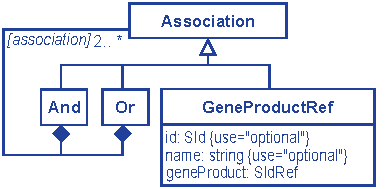
\includegraphics[width=10cm]{images/v2harmony_fbc_association.pdf}\\
  \caption{A UML representation of the \FBCPackage \Association and derived
	classes. The [association] element name is the name of the class, de-capitalized. In this case, the possible values are "and", "or", or "geneProductRef". For a complete description see \ref{fig:fbc_uml} as well as \ref{conventions} for conventions related to this figure.}
  \label{fig:fbc_uml_ass}
\end{figure}

\subsection{The \FBC \class{GeneProductRef} class}
\label{geneproductref-class}

The \FBCPackage defines a \GeneProductRef class that references
a \GeneProduct declared in \ListOfGeneProducts, a child of
\Model (see \ref{geneproduct-class}). It is derived from an \Association and thereby inherits the \SBase attributes \token{metaid} and \token{sboTerm}, as well as the subcomponents for \Annotation and \Notes as described in \ref{fig:fbc_uml_ass}.

\paragraph{The \token{id} and \token{name} attributes}
A \GeneProductRef has two optional attributes: \token{id} an attribute of
type \primtype{SId} and \token{name} an attribute of type \primtype{string}.

%\paragraph{The \token{species} attribute}
%The optional attribute \token{species} attribute of type \primtype{SIdRef} can  refer to a \Species element defined within the enclosing model. The intention here is to allow gene--protein associations to be linked to \Species which may represent them in the model thus bridging two conceptually different (yet equally valid) ways of representing such relations. This attribute should be used in conjunction with the extended \Species attribute \token{isGene} (see \ref{species-class-ga} for details).

\paragraph{The \token{geneProduct} attribute}
The required \token{geneProduct} attribute of type %\primtype{FbcSIdRef}
\primtype{SIdRef}
references a \GeneProduct element declared in the \ListOfGeneProducts.
\pagebreak
\subsection{The \FBC \class{And} class}
\label{and-class}

The \FBCPackage defines an \GeneAnd class that is derived from
an \Association and thereby inherits the \SBase attributes \token{metaid}
and \token{sboTerm}, as well as the subcomponents for \Annotation and
\Notes as described in \ref{fig:fbc_uml_ass}. This class represents a
set of two or more associations that are related in an order independent
\emph{`and'} relationship.

\paragraph{The \token{elements} element}
Each \GeneAnd must contain two or more instances (not necessarily of
the same type) of any \Association subclass (\GeneAnd, \GeneOr,
\GeneProductRef).

\exampleFile{examples/v2harmony-spec-example1-geneand.txt}

\subsection{The \FBC \class{Or} class}
\label{or-class}

The \FBCPackage defines an \GeneOr class that represents a gene
(or gene product) and is derived from an \Association and thereby inherits
the \SBase attributes \token{metaid} and \token{sboTerm}, as well as the
subcomponents for \Annotation and \Notes as described in \ref{fig:fbc_uml_ass}.
This class represents a set of two or more \Association elements related
in an order independent \emph{`or'} relationship.

\paragraph{The \token{elements} element}
Each \GeneOr must contain two or more instances (not necessarily of the
same type) of any \Association subclass (\GeneAnd, \GeneOr, \GeneProductRef).
%
\exampleFile{examples/v2harmony-spec-example1-geneor.txt}

% -*- TeX-master: "main"; fill-column: 72 -*-

\subsection{The \FBC \class{UserDefinedConstraint} class}
\label{userdefinedconstraint-class}

\newtxt{The \FBC \UserDefinedConstraint class is derived from \SBML \SBase and inherits \token{metaid} and \token{sboTerm}, as well as the subcomponents for \Annotation and \Notes. It's purpose is to allow the definition of non-stoichiometric constraints, that is, constraints that are not defined by the stoichiometrically coupled reaction network. In order to achieve this a new class of constraint is defined, the \UserDefinedConstraint.}
%
\begin{figure}[ht]
  \centering
  % Requires \usepackage{graphicx}
  %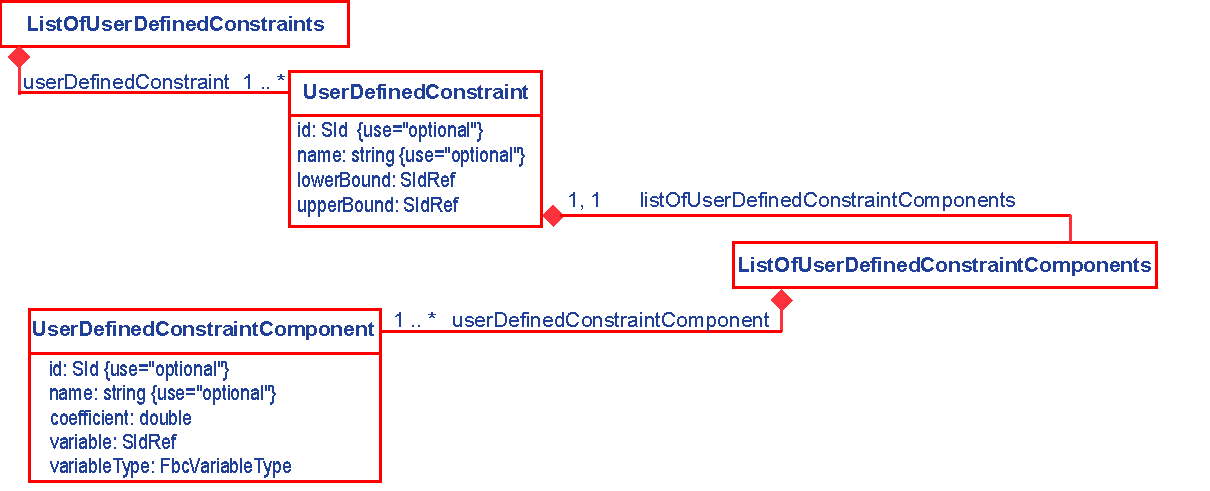
\includegraphics[width=6cm]{images/fbc_v3_uml_userdefinedconstraint.pdf}\\
  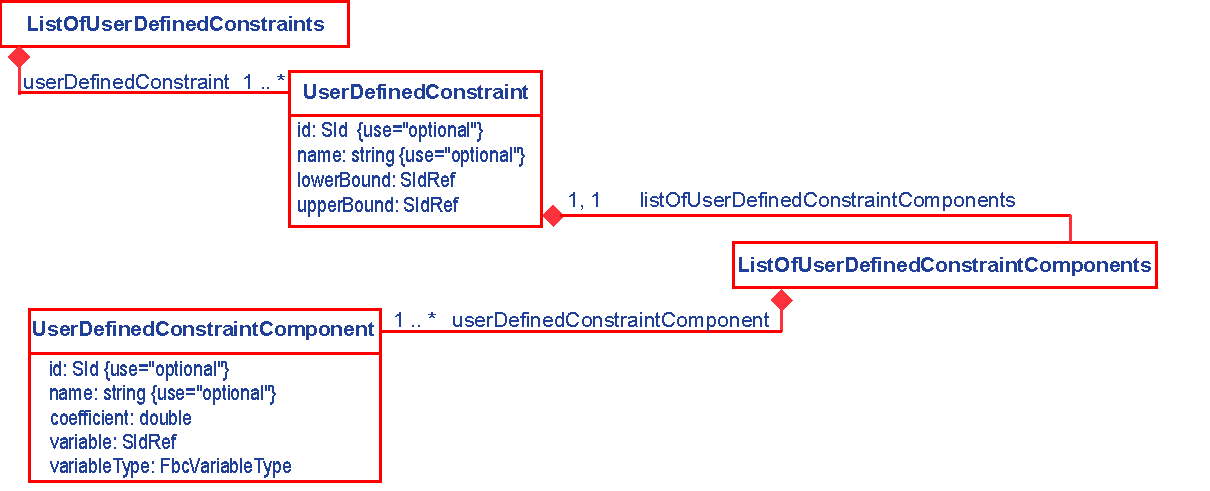
\includegraphics[width=0.9\textwidth]{images/fbc_v3_uml_userdefinedconstraint.pdf}\\
  \caption{A UML representation of the \SBML \Model class extended in
  the \FBCPackage by the \ListOfUserDefinedConstraints. See \ref{conventions} for conventions related to this figure.}
  \label{fig:fbc_v3_uml_user_constraints}
\end{figure}


\newtxt{Analogous to the attributes described in the \Reaction class (\ref{reaction-class-ga}), the \token{lowerBound} and \token{upperBound} define the upper and lower bounds of the \UserDefinedConstraint, such that:}
%
\begin{equation}\label{eqn:userderfinedconstraint}
\centering
  \token{lowerBound} \leq \UserDefinedConstraint \leq \token{upperBound}
\end{equation}

%
\newtxt{The \UserDefinedConstraint contains a \ListOfUserDefinedConstraintComponents representing a linear combination of \UserDefinedConstraintComponent{s}. Similar to a \FluxObjective each \UserDefinedConstraintComponent contains a coefficient--variable pair where the \token{coefficient} refers to a constant \Parameter. Furthermore, the \UserDefinedConstraintComponent \token{variable} attribute may either refer to a \Reaction or to a non-constant \Parameter, thus allowing the use of non-reaction, artificial, variables. See the attribute descriptions for more detail.}

\paragraph{The \token{id} and \token{name} attributes}
\newtxt{A \UserDefinedConstraint has an optional \token{id} of type
\primtype{SId} and an optional attribute \token{name} of type \primtype{string}.}

\paragraph{The \token{lowerBound} attribute}
\newtxt{The required \token{lowerBound} attribute contains an \primtype{SIdRef} that references a \Parameter which contains the lower boundary value of the \UserDefinedConstraint.}

\paragraph{The \token{upperBound} attribute}
\newtxt{The required \token{upperBound} attribute contains an \primtype{SIdRef} that references a \Parameter which contains the upper boundary value of the \UserDefinedConstraint.}

\paragraph{The \token{listOfUserDefinedConstraintComponents} element}
\label{listofuserdefinedconstraintcomponents-class}

\newtxt{The element \token{listOfUserDefinedConstraintComponents} which contains a
\ListOfUserDefinedConstraintComponents is derived from and functions like a typical \SBML
\textsf{\textbf{ListOf\rule{0.15in}{0.5pt}}} class with the restriction that it
must contain one or more elements of type \UserDefinedConstraintComponent (see \ref{userdefinedconstraintcomponent-class}).This implies that if a \UserDefinedConstraint is defined there should be at least one \UserDefinedConstraintComponent contained in a \ListOfUserDefinedConstraintComponents.}

\subsection{The \FBC \class{UserDefinedConstraintComponent} class}
\label{userdefinedconstraintcomponent-class}

\newtxt{The \FBC \UserDefinedConstraintComponent class is derived from \SBML \SBase and inherits
\token{metaid} and \token{sboTerm}, as well as the subcomponents for
\Annotation and \Notes. The \UserDefinedConstraintComponent class is a relatively simple container for a variable and a variable type specifier which is weighted by a signed coefficient.}

\paragraph{The \token{id} and \token{name} attributes}
\newtxt{An \UserDefinedConstraintComponent has an optional \token{id} of type \primtype{SId} and an optional attribute \token{name} of type \primtype{string}.}

\paragraph{The \token{coefficient} attribute}
\newtxt{The required \token{coefficient} attribute contains an \primtype{SIdRef} that is restricted to reference only a \Parameter which holds the coefficient value. In \textbf{strict} mode a \Parameter whose \primtype{SId} is referenced by a \token{coefficient}, has to be set as \token{constant} and not take the value \val{NaN} or \val{$\pm$INF}.}

\paragraph{The \token{variable} attribute}
\newtxt{The required \token{variable} attribute contains an \primtype{SIdRef} that is restricted to reference the \primtype{SId} of either a \Reaction or non-constant \Parameter. In \textbf{strict} mode such a non-constant \Parameter whose \primtype{SId} is referenced by a \UserDefinedConstraintComponent \token{variable} attribute may not be referenced by any \UserDefinedConstraintComponent \token{coefficient}, \UserDefinedConstraint \token{lowerBound} \& \token{upperBound} or \Reaction \token{lowerFluxBound} \& \token{upperFluxBound} attribute.}

\paragraph{The \token{variableType} attribute}
\newtxt{The required \token{variableType} attribute contains a \primtype{FbcVariableType} that indicates whether a variable should be considered as \val{linear} or \val{quadratic}.}

\paragraph{An example of encoding two user defined constraints in \SBML}
\newtxt{The following example illustrates the encoding of two \UserDefinedConstraint{s}. The first uses only \Reaction{s} as variables, while the second introduces an artificial, non-constant, \Parameter as a variable.}
\begin{eqnarray}
% \nonumber to remove numbering (before each equation)
  RGLX - RBTK  &=& 5 \\
  2\cdot p1var - RGDP &\geq& 2
\end{eqnarray}
\exampleFile{examples/ex-v3-userdefinedconstraints.txt}

\newpage
\subsection{The \FBC \class{ListOfKeyValuePairs} class}
\label{listofkeyvaluepairs-class}

The \ListOfKeyValuePairs, see \ref{fig:fbc_v3_uml_keyvalue} for details, forms the basis of a controlled annotation defined by the \FBCPackage. This element defines a `structured note' or `descriptive list' of keys and associated values.
%
\exampleFile{examples/ex-v3-kvp1.txt}
%
As such it is analogous to the official \SBML RDF annotation used to support MIRIAM annotations, as defined in the \SBML specification documents. When an annotation that declares the \token{xmlns} \token{http://sbml.org/fbc/keyvaluepair} then it must have the format specified here. Tools may choose to support reading and interpreting the content as described, but may optionally ignore the annotation and merely round trip it with any other third party annotations. As is the case with the RDF/MIRIAM annotations, support for \ListOfKeyValuePairs will be included in the \SBML support libraries.
%
\begin{figure}[ht]
  \centering
  % Requires \usepackage{graphicx}
  %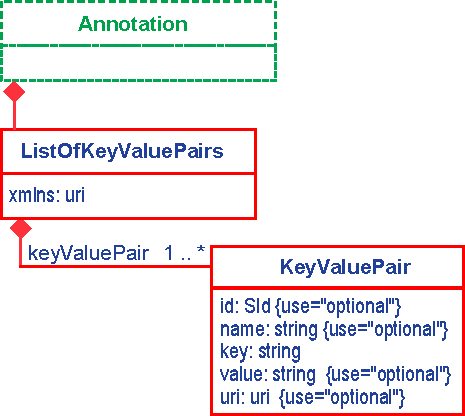
\includegraphics[width=6cm]{images/fbc_v3_uml_keyvalue.pdf}\\
  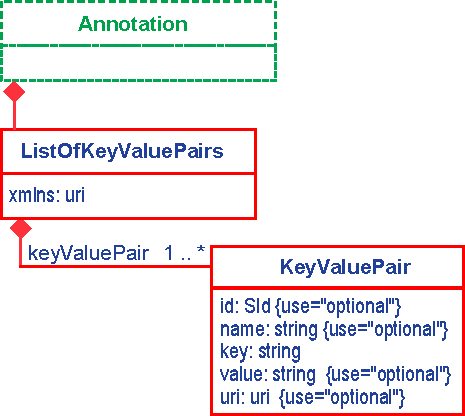
\includegraphics[width=0.6\textwidth]{images/fbc_v3_uml_keyvalue.pdf}\\
  \caption{A UML representation of the \SBML \SBase class extended in
  the \FBCPackage by the \protect{\ListOfKeyValuePairs}. See \ref{conventions} for conventions related to this figure.}
  \label{fig:fbc_v3_uml_keyvalue}
\end{figure}
%
The \ListOfKeyValuePairs functions like a typical \SBML \textsf{\textbf{ListOf\rule{0.15in}{0.5pt}}} class with the restriction that it must contain one or more elements of type \KeyValuePair (see \ref{keyvaluepair-class}). In addition it defines a single mandatory attribute, \token{xmlns}, which identifies the annotation as belonging to the \FBCPackage.

\paragraph{The \token{xmlns} attribute}
The \token{xmlns} is a mandatory component of the \ListOfKeyValuePairs, is of the type \primtype{uri} and must have the value \token{http://sbml.org/fbc/keyvaluepair}.


\subsection{The \FBC \class{KeyValuePair} class}
\label{keyvaluepair-class}

The \FBC \KeyValuePair class' sole purpose is to define a key--value pair with an optional extended key definition.

The \KeyValuePair defines a single mandatory attribute the \token{key} as well as four optional attributes: \token{value}, \token{uri}, \token{id} and \token{name}.

\paragraph{The \token{id} and \token{name} attributes}
A \KeyValuePair has two optional attributes: \token{id} an attribute of
type \primtype{SId} and \token{name}, an attribute of type \primtype{string}.

\paragraph{The \token{key} attribute}
The \token{key} is the mandatory component of the \KeyValuePair pair and is of type \primtype{string}. It has the special property that every \token{key} in an enclosing \ListOfKeyValuePairs must be unique.

\paragraph{The \token{value} attribute}
The optional \token{value} attribute is of \primtype{string} and contains the value associated with a particular \token{key}. If not present, the \KeyValuePair is defined as having no value.

\paragraph{The \token{uri} attribute}
The optional attribute \token{uri} is of type \primtype{uri}. This attribute identifies a resource that defines the associated \token{key} component of the \KeyValuePair, see~\ref{table:kvpuris} for examples. As a best practice, it is highly recommended that all tools implementing a \KeyValuePair also implement support for the \token{uri} attribute.
%
\begin{table}
  \centering
  \begin{tabular}{lll}
  \toprule
   \textbf{Type} & \textbf{Example} & \textbf{Description} \\
  \midrule
   \textbf{urn} & urn:tinyurl.com:example:kvp & a tool specific namespace declaration \\
   \textbf{url} & \url{https://github.com/sbmlteam} & a url identifying a set of \token{key} definitions\\
   \bottomrule
  \end{tabular}
   \caption{Examples of how the \token{uri} attrbitue can be used to identify \token{key} definitions by \textbf{urn} or \textbf{url}.}\label{table:kvpuris}
\end{table}




















%\newpage
%\section{\FBC version 3: updated HARMONY 2020}

%The proposed \FBCPackage version~3 extends the definition of the \FluxObjective, extends the definition of the \token{chemicalFormula}, redefines \token{charge} as a double, defines a \UserDefinedConstraint and adds a generic \KeyValuePair annotation.
%%
%\begin{quote}
% \newtxt{\textbf{The extensions and modifications contained in this document are proposed as version 3 of the \FBCPackage. This proposal is been formulated through open discussions on the \FBC PWG mailing list and intense discussion during HARMONY 2018 and HARMONY 2020. }}
%\end{quote}
%%
%\begin{quote}
%  \newtxt{At HARMONY 2020 it was decided that the name `UserDefinedConstraint' should be changed to something else.}
%\end{quote}
%
%%
%Please note that where specification text (or UML) has been modified and diverges from the \FBCPackage version~2 specification, it has been colored \newtxt{red}.
%
%\begin{figure}[ht!]
%  \centering
%  % Requires \usepackage{graphicx}
%  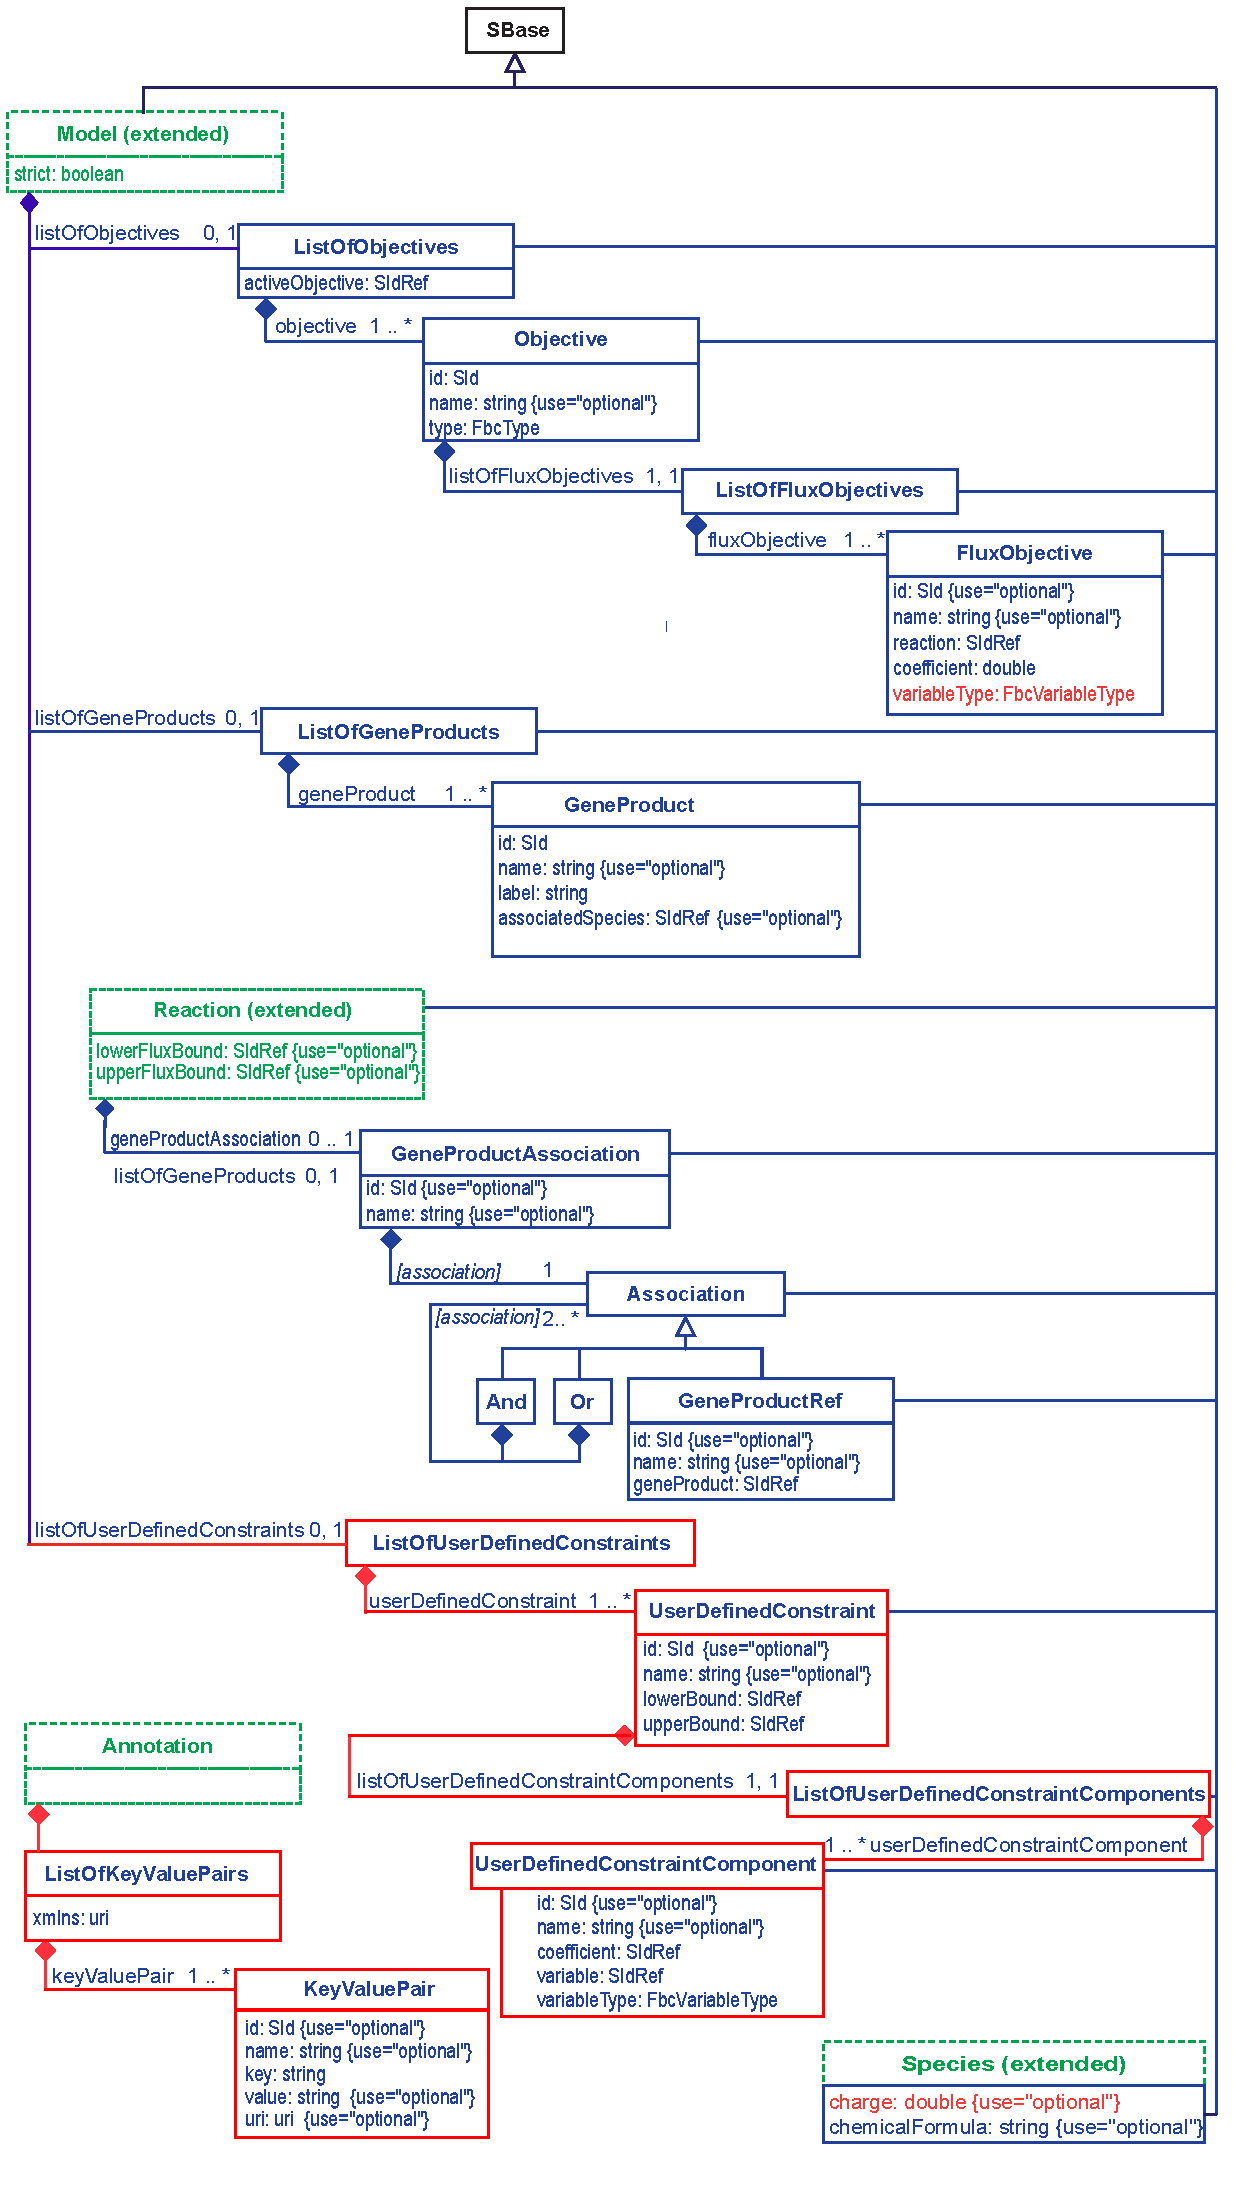
\includegraphics[height=0.85\textheight]{images/fbc_uml_v3.pdf}\\
%  \caption{A UML representation of the \FBCPackage version three. Derived from \SBase, most\FBC classes inherit support for constructs such as SBML \Notes and \Annotation's. The [association] element name is the name of the class, de-capitalized. In this case, the possible values are "and", "or", or "geneProductRef". See \ref{conventions} for conventions related to this figure. The individual classes are further discussed in the text.}
%  \label{fig:fbc_uml_v3}
%\end{figure}

%\subsection{The extended \class{SBase} class}
%\label{sbase-class-kv}

%\subsection{The extended \class{Model} class (updates specification \ref{model-class})}
%\label{model-class-kv}
%\label{listoffluxbounds-class}



%\subsubsection{Type \primtypeNC{FbcVariableType}}
%\label{primtype-fbcvariabletype}
%
%The \FBCPackage defines a new enumerated type \primtype{FbcVariableType} which
%represents the index of a variable that occurs in either the \FluxObjective or \UserDefinedConstraintComponent. It contains the following two values, \val{linear} or \val{quadratic}.


%\subsubsection{Type \primtypeNC{FbcUCCVariableType}}
%\label{primtype-fbcuserdefinedconstraintvariabletype}
%
%The \FBCPackage defines a new enumerated type \primtype{FbcUCCVariableType} which
%represents the index of a variable that occurs in a user defined constraint. It can have one
%of the following two values \val{linear} or \val{quadratic}.

%The \SBML \Model class is extended by a \token{listOfUserDefinedConstraints} of which it may contain at most one, see  \ref{fig:fbc_v3_uml_user_constraints}.
%
%\subsubsection{The \FBC \class{listOfUserDefinedConstraints}}
%\label{listofuserdefinedconstraints-class}
%
%As shown in \ref{fig:fbc_v3_uml_user_constraints} the \ListOfUserDefinedConstraints is derived from \SBase and inherits the attributes \token{metaid} and \token{sboTerm}, as well as
%the subcomponents for \Annotation and \Notes. The \ListOfUserDefinedConstraints must contain at least one \UserDefinedConstraint (defined in \ref{userdefinedconstraint-class}).

%\pagebreak
%
%\subsection{The extended \class{Species} class (updates specification \ref{species-class})}
%
%The \FBCPackage extends the \sbmlthreecore \Species class with the addition
%of two attributes \token{charge} and \token{chemicalFormula}.
%%
%\begin{figure}[h]
%  \centering
%  % Requires \usepackage{graphicx}
%  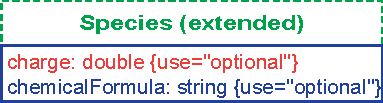
\includegraphics[width=6cm]{images/v3harmony_fbc_species.pdf}\\
%  \caption{A UML representation of the extended \SBML \Species class used in
%  the \FBCPackage. See \ref{conventions} for conventions related to this
%  figure.}
%  \label{fig:fbc_uml_species_v3}
%\end{figure}

%\paragraph{The \token{charge} attribute}
%
%\newtxt{The optional attribute charge contains a signed double referring to the Species object’s charge (in terms of electrons, not the SI unit coulombs). Note, that unlike FBC versions one and two a \Species may, for the purposes of charge, be interpreted as a pseudoisomer or aggregate molecule and may assume a non-integer value. Non-integer charges should be used with caution as their use may have unintended side-effects, for example, with respect to the accuracy of reaction balancing.}
%
%%The optional attribute \token{charge} which contains a signed
%%\primtype{integer} referring to the \Species object's charge and is
%%defined as it was in the \SBML Level 2 Version 1 specification
%%: \textit{``The optional field charge takes an integer indicating
%%the charge on the species (in terms of electrons, not the SI unit coulombs).''}
%
%\paragraph{The \token{chemicalFormula} attribute}
%\label{chemicalFormula-attribute}
%
%The optional attribute \token{chemicalFormula} containing a \primtype{string} that represents the \Species objects elemental composition.
%%
%\exampleFile{examples/ex-v3-species.txt}
%%
%\newtxt{While there are many ways of referring to an elemental composition, the purpose of the \token{chemicalFormula} attribute is to enable reaction balancing and validation, something of particular importance in constraint-based models.}
%
%\newtxt{The format of the \token{chemicalFormula} should, whenever possible, consist only of atomic names
%(as in the Periodic Table). Similarly, for enhanced inter-operability, the element order should be arranged according to the Hill system (see \ref{table:hill2})} \citep{hillsystem, hillwikipedia}.
%%
%\begin{table}[h!]
%  \begin{tabular}{ccc}
%    % after \\: \hline or \cline{col1-col2} \cline{col3-col4} ...
%     $H_{2}O_{4}S$ & $C_{2}H_{5}Br$ & $BrH$ \\
%     $C_{10}H_{12}N_{5}O_{13}P_{3}$ & $CH_{3}I$ & $CH_{4}$  \\
%  \end{tabular}
%  \caption{Examples of chemical formulas written using the Hill System. As
%	described in \ref{chemicalFormula-attribute}}\label{table:hill2}
%\end{table}
%%
%\newtxt{Using this notation the number of carbon atoms in a molecule is indicated first, followed by the number of hydrogen atoms and then the number of all other chemical elements in alphabetical order. When the formula contains no carbon; all elements, including hydrogen, are listed alphabetically. Where there is more than a single atom present, this is indicated with an integer that follows the element symbol.}
%
%\newtxt{However, in certain situations it does become necessary to use a generic symbol in a user defined compound. For example, such symbols can include \textsf{R} and \textsf{X} and have the general form of a single capital letter followed by zero or more lowercase letters.}
%%
%\begin{table}[h!]
%  \begin{tabular}{ccc}
%    % after \\: \hline or \cline{col1-col2} \cline{col3-col4} ...
%     $RCONH_{2}$ & $RCOX$ & $C_{2}H_{4}O_{2}(CH_{2})_{n}$ \\
%  \end{tabular}
%  \caption{Examples of chemical formulas written using allowed non-Hill symbols, as described in \ref{chemicalFormula-attribute}.}\label{table:non-hill}
%\end{table}
%%
%\newtxt{In addition, the undefined parenthesised group index $(\ldots)_n$ may also be used. Note that in this case only the subscript $n$ is allowed, integer values $(\ldots)_2$ and expressions such as $(\ldots)_{n-1}$ are considered invalid.}
%
%\newtxt{However, the use of \textsf{R}, \textsf{X} and $(\ldots)_n$ is not advised, as any \Reaction in which such a \Species occurs cannot necessarily be balanced. Therefore, any \token{chemicalFormula} that contains any of the aforementioned, non-Hill compatible symbols will raise a `best practices' warning on model validation.}

%\subsection{The \FBC \class{FluxObjective} class}
%
%The \FBC \FluxObjective class is derived from \SBML \SBase and inherits
%\token{metaid} and \token{sboTerm}, as well as the subcomponents for
%\Annotation and \Notes.
%%
%\begin{figure}[ht]
%  \centering
%  % Requires \usepackage{graphicx}
%  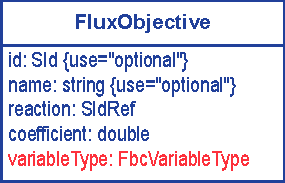
\includegraphics[width=6cm]{images/fbc_v3_uml_fobj.pdf}\\
%  \caption{A UML representation of the \FBCPackage \FluxObjective class. For a complete description see \ref{fig:fbc_uml} as well as \ref{conventions} for conventions related to this figure.}
%  \label{fig:fbc_uml_userdefinedconstraint}
%\end{figure}
%%
%The \FluxObjective class is a relatively simple container for a model
%variable that can be expressed as a `linear' or `quadratic', weighted by a signed linear coefficient.
%
%\paragraph{The \token{id} and \token{name} attributes}
%A \FluxObjective has two optional attributes: \token{id} an attribute of
%type \primtype{SId} and \token{name} an attribute of type \primtype{string}.
%
%\paragraph{The \token{reaction} and \token{coefficient} attributes}
%The required \token{reaction} is of type \primtype{SIdRef} and is restricted
%to refer only to a \Reaction while the \token{coefficient} attribute
%holds a \primtype{double} referring to the coefficient that this \FluxObjective
%takes in the enclosing \Objective.
%
%\newtxt{\paragraph{The \token{variableType} attribute}
%The required \token{variableType} attribute contains a \primtype{FbcVariableType} that
%represents the index to which a variable is raised in a \FluxObjective. For example, where $J_{x}$ represents a steady-state flux the \primtype{FbcVariableType} defines either a \val{linear}, $J^1_x$ or \val{quadratic}, $J^2_x$ term.}
%
%\paragraph{Flux objectives: example code}
%\newtxt{An objective with purely linear terms in LP format:} \verb"Maximize: 1 R1 + 2 R2"
%%
%\exampleFile{examples/ex-v3-fluxobjective-linear.txt}
%%
%\newtxt{Similarly, an objective with a quadratic term in LP format:} \verb"Minimize: 1 R1 + [4 R2^2]/2"
%%
%\exampleFile{examples/ex-v3-fluxobjective.txt}
%
%\paragraph{Units}
%As described above the linear \FluxObjective defined here as $n\cdot J$ where
%the \token{coefficient} ($n$) is dimensionless and the \token{value} ($J$)
%takes the units of the \token{reaction} flux i.e.,~``extent per time''.
%\newtxt{Therefore, the \token{linear} \FluxObjective, ($n\cdot J$)  has the unit $\frac{extent}{time}$ where the units of reaction ``extent'' and ``time'' are defined globally. Analogously, in the case of a \token{quadratic} \FluxObjective, $n\cdot J^{2}$ this would be $\frac{extent^{2}}{time^{2}}$}.



%\subsection{The \FBC \class{UserDefinedConstraint} class}
%\label{userdefinedconstraint-class}
%
%The \FBC \UserDefinedConstraint class is derived from \SBML \SBase and inherits
%\token{metaid} and \token{sboTerm}, as well as the subcomponents for
%\Annotation and \Notes. It's purpose is to define non-stoichiometric constraints, that is  constraints that are not necessarily defined by the stoichiometrically coupled reaction network. In order to achieve we defined a new type of linear constraint, the \UserDefinedConstraint.
%%
%\begin{figure}[ht]
%  \centering
%  % Requires \usepackage{graphicx}
%  %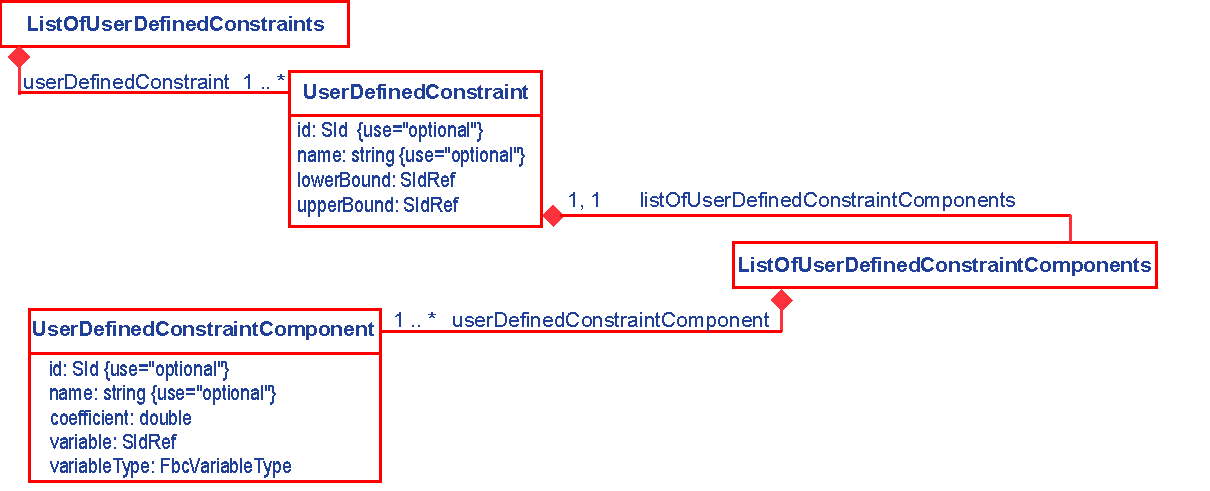
\includegraphics[width=6cm]{images/fbc_v3_uml_userdefinedconstraint.pdf}\\
%  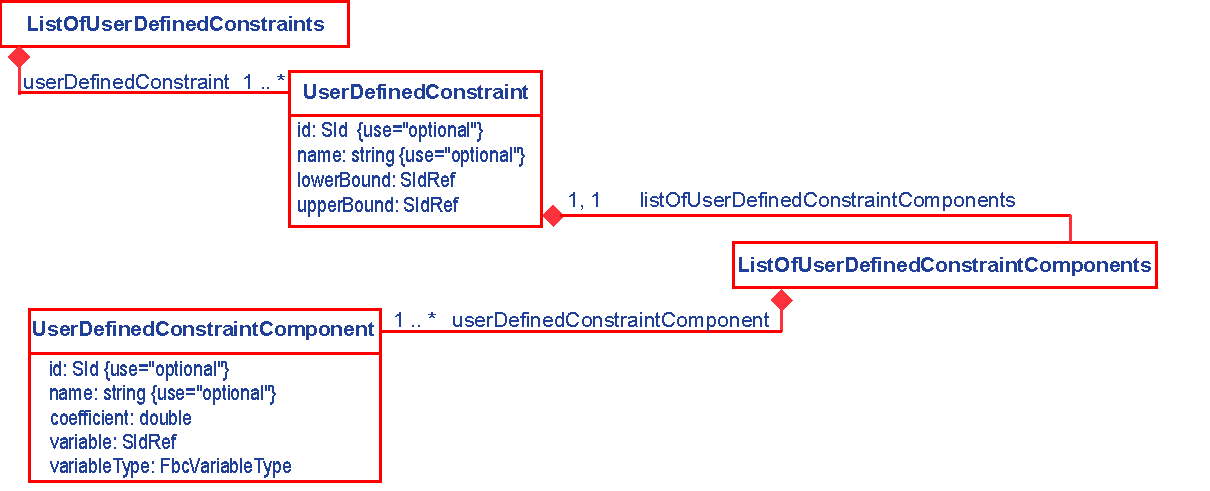
\includegraphics[width=0.9\textwidth]{images/fbc_v3_uml_userdefinedconstraint.pdf}\\
%  \caption{A UML representation of the \SBML \Model class extended in
%  the \FBCPackage by the \ListOfUserDefinedConstraints. See \ref{conventions} for conventions related to this figure.}
%  \label{fig:fbc_v3_uml_user_constraints}
%\end{figure}
%
%
%Analogous to the attributes described in \ref{reaction-class-ga} the \token{lowerBound} and \token{upperBound} form the boundaries of the \UserDefinedConstraint.
%%
%\begin{eqnarray}
%% \nonumber to remove numbering (before each equation)
%  \UserDefinedConstraint &=& \token{value} \\
%  \UserDefinedConstraint &\geq& \token{lowerBound value} \\
%  \UserDefinedConstraint &\leq& \token{upperBound value}
%\end{eqnarray}
%%
%Defining either an equality if both \token{lowerBound} and \token{upperBound} refere to the same parameter (Equation~4) or set of inequalities (Equations 4 and 5).
%
%The \UserDefinedConstraint contains a \ListOfUserDefinedConstraintComponents representing a linear combination of \UserDefinedConstraintComponent{s}. Similar to a \FluxObjective each \UserDefinedConstraintComponent contains a coefficient--variable pair where the \token{coefficient} refers to a \Parameter. In addition to a \Reaction a \UserDefinedConstraintComponent allows the \token{variable} to refer to non-constant \Parameter thus allowing the definition of non-reaction, artificial, variables.
%
%\paragraph{The \token{id} and \token{name} attributes}
%A \UserDefinedConstraint has an optional \token{id} of type
%\primtype{SId} and an optional attribute \token{name} of type \primtype{string}.
%
%\paragraph{The \token{lowerBound} attribute}
%The required \token{lowerBound} attribute contains an \primtype{SIdRef} that references a \Parameter which contains the lower boundary value of the \UserDefinedConstraint.
%
%\paragraph{The \token{upperBound} attribute}
%The required \token{upperBound} attribute contains an \primtype{SIdRef} that references a \Parameter which contains the upper boundary value of the \UserDefinedConstraint.
%
%\paragraph{The \token{listOfUserDefinedConstraintComponents} element}
%\label{listofuserdefinedconstraintcomponents-class}
%
%The element \token{listOfUserDefinedConstraintComponents} which contains a
%\ListOfUserDefinedConstraintComponents is derived from and functions like a typical \SBML
%\textsf{\textbf{ListOf\rule{0.15in}{0.5pt}}} class with the restriction that it
%must contain one or more elements of type \UserDefinedConstraintComponent (see \ref{userdefinedconstraintcomponent-class}).
%This implies that if a \UserDefinedConstraint is defined there should be at least
%one \UserDefinedConstraintComponent contained in a \ListOfUserDefinedConstraintComponents.
%
%\subsection{The \FBC \class{UserDefinedConstraintComponent} class}
%\label{userdefinedconstraintcomponent-class}
%
%The \FBC \UserDefinedConstraintComponent class is derived from \SBML \SBase and inherits
%\token{metaid} and \token{sboTerm}, as well as the subcomponents for
%\Annotation and \Notes. The \UserDefinedConstraintComponent class is a relatively simple container for a variable and a variable type specifier which is weighted by a signed coefficient.
%
%\paragraph{The \token{id} and \token{name} attributes}
%An \UserDefinedConstraintComponent has an optional \token{id} of type \primtype{SId} and an optional attribute \token{name} of type \primtype{string}.
%
%\paragraph{The \token{coefficient} attribute}
%The required \token{coefficient} attribute contains an \primtype{SIdRef} that is restricted to reference only a constant \Parameter which holds the coefficient value. In \textbf{strict} mode a \Parameter whose \primtype{SId} is referenced by a \token{coefficient}, as in the case of a \FluxObjective \token{coefficient}, has to be constant and not take the value NaN or $\pm$inf.
%
%\paragraph{The \token{variable} attribute}
%The required \token{variable} attribute contains an \primtype{SIdRef} that is restricted to reference the \primtype{SId} of either a \Reaction or a non-constant \Parameter. Conversely, if such non-constant \Parameter's \primtype{SId} is referenced by a \UserDefinedConstraintComponent's \token{variable} attribute it may not be referenced by any \token{coefficient}, \token{lowerFluxBound} or \token{upperFluxBound} attribute.
%
%\paragraph{The \token{variableType} attribute}
%The required \token{variableType} attribute contains a \primtype{FbcVariableType} that indicates whether a variable should be considered as `linear' or `quadratic'.
%
%\paragraph{User constraints: example code}
%The following example illustrates the encoding of the following two \UserDefinedConstraint{s}:
%\begin{eqnarray}
%% \nonumber to remove numbering (before each equation)
%  RGLX - RXLG  &=& 5 \\
%  2\cdot Avar - RGDP &\geq& 2
%\end{eqnarray}
%\exampleFile{examples/ex-v3-userdefinedconstraints.txt}





%\subsection{The \FBC \class{ListOfKeyValuePairs} class}
%\label{listofkeyvaluepairs-class}
%
%The \ListOfKeyValuePairs, see \ref{fig:fbc_v3_uml_keyvalue} for details, forms the basis of a controlled annotation defined by the \FBCPackage. This element defines a `structured note' or `descriptive list' of keys and associated values.
%%
%\exampleFile{examples/ex-v3-kvp1.txt}
%%
%As such it is analogous to the official \SBML RDF annotation used to support MIRIAM annotations, as defined in the \SBML specification documents. When an annotation that declares the \token{xmlns} \token{http://sbml.org/fbc/keyvaluepair} then it must have the format specified here. Tools may choose to support reading and interpreting the content as described, but may optionally ignore the annotation and merely round trip it with any other third party annotations. As is the case with the RDF/MIRIAM annotations, support for \ListOfKeyValuePairs will be included in the \SBML support libraries.
%%
%\begin{figure}[ht]
%  \centering
%  % Requires \usepackage{graphicx}
%  %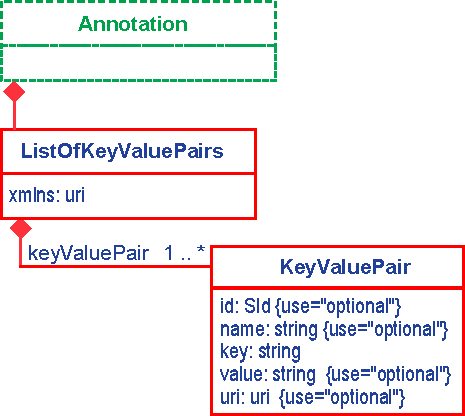
\includegraphics[width=6cm]{images/fbc_v3_uml_keyvalue.pdf}\\
%  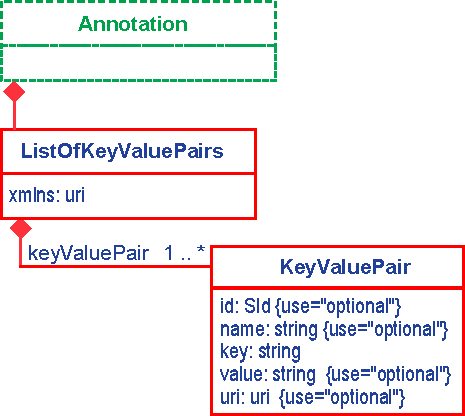
\includegraphics[width=0.6\textwidth]{images/fbc_v3_uml_keyvalue.pdf}\\
%  \caption{A UML representation of the \SBML \SBase class extended in
%  the \FBCPackage by the \protect{\ListOfKeyValuePairs}. See \ref{conventions} for conventions related to this figure.}
%  \label{fig:fbc_v3_uml_keyvalue}
%\end{figure}
%%
%The \ListOfKeyValuePairs functions like a typical \SBML \textsf{\textbf{ListOf\rule{0.15in}{0.5pt}}} class with the restriction that it must contain one or more elements of type \KeyValuePair (see \ref{keyvaluepair-class}). In addition it defines a single mandatory attribute, \token{xmlns}, which identifies the annotation as belonging to the \FBCPackage.
%
%\paragraph{The \token{xmlns} attribute}
%The \token{xmlns} is a mandatory component of the \ListOfKeyValuePairs, is of the type \primtype{uri} and must have the value \token{http://sbml.org/fbc/keyvaluepair}.
%
%
%\subsection{The \FBC \class{KeyValuePair} class}
%\label{keyvaluepair-class}
%
%The \FBC \KeyValuePair class' sole purpose is to define a key--value pair with an optional extended key definition.
%
%The \KeyValuePair defines a single mandatory attribute the \token{key} as well as four optional attributes: \token{value}, \token{uri}, \token{id} and \token{name}.
%
%\paragraph{The \token{id} and \token{name} attributes}
%A \KeyValuePair has two optional attributes: \token{id} an attribute of
%type \primtype{SId} and \token{name}, an attribute of type \primtype{string}.
%
%\paragraph{The \token{key} attribute}
%The \token{key} is the mandatory component of the \KeyValuePair pair and is of type \primtype{string}. It has the special property that every \token{key} in an enclosing \ListOfKeyValuePairs must be unique.
%
%\paragraph{The \token{value} attribute}
%The optional \token{value} attribute is of \primtype{string} and contains the value associated with a particular \token{key}. If not present, the \KeyValuePair is defined as having no value.
%
%\paragraph{The \token{uri} attribute}
%The optional attribute \token{uri} is of type \primtype{uri}. This attribute identifies a resource that defines the associated \token{key} component of the \KeyValuePair, see~\ref{table:kvpuris} for examples. As a best practice, it is highly recommended that all tools implementing a \KeyValuePair also implement support for the \token{uri} attribute.
%%
%\begin{table}
%  \centering
%  \begin{tabular}{lll}
%  \toprule
%   \textbf{Type} & \textbf{Example} & \textbf{Description} \\
%  \midrule
%   \textbf{urn} & urn:tinyurl.com:example:kvp & a tool specific namespace declaration \\
%   \textbf{url} & \url{https://tinyurl.com/ybyr7b62} & a url identifying a set of \token{key} definitions\\
%   \bottomrule
%  \end{tabular}
%   \caption{Examples of how the \token{uri} attrbitue can be used to identify \token{key} definitions by \textbf{urn} or \textbf{url}.}\label{table:kvpuris}
%\end{table}






% -*- TeX-master: "main"; fill-column: 72 -*-

\section{Illustrative examples of the \FBC syntax}
\label{examples}

This section contains a worked example showing the encoding of a model suitable for Flux Balance Analysis using the \FBCPackage.

\subsection{Example one: the basic \FBC syntax}
\label{examples1}
\subsubsection{Kinetic model description}
\begin{figure}[h]
  \centering
  % Requires \usepackage{graphicx}
  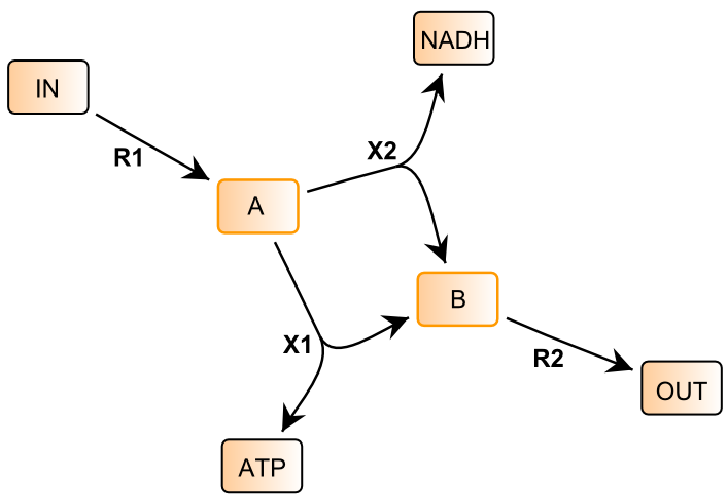
\includegraphics[width=8cm]{examples/spec-example1.pdf}\\
  \caption{\FBC syntax example: a simple four reaction pathway. The
  reactions are \textit{R1}, \textit{R2}, \textit{X1}, \textit{X2} with
  fixed species \textit{IN}, \textit{OUT}, \textit{ATP}, \textit{NADH} and
  variable species \textit{A}, \textit{B}.}
  \label{fig:example1}
\end{figure}

As shown in \ref{fig:example1} this example is a simple four reaction
pathway that transforms metabolite \textit{IN} to \textit{OUT}. The
model was created and analyzed using the \textsf{SBW Flux Balance} \FBC
implementation and CBMPy \citep{sbwfba, cbmpy}. In \SBML each reaction is represented as a chemical process transforming reactants to products, e.g. reaction
\textit{R1} is encoded in XML as (see also the complete example provided
at the end of this section):


%
\exampleFile{examples/spec-example1-reaction.txt}
%
Using the reagent identity and stoichiometry it is possible to compactly
describe this network in terms of its reaction stoichiometry as shown in
\ref{tble:ex1nmat} where each reaction is represented as a column. Each row in the stoichiometric matrix represents the differential equation describing the change of a variable \Species. In \SBML such variable \Species have the attribute \token{boundaryCondition} set to \val{false}. This is in contrast to ``fixed species'' (where the attribute \token{boundaryCondition} is set to \val{true}) which do not appear in the stoichiometric matrix. Please see the \sbmlthreecore specification for more details.

\begin{table}[h]
  \centering
    \begin{tabular}{c|cccc}
          & R1 & R2 & X1 & X2 \\ \hline
        A & 1 &  0 & -1 & -1 \\
        B & 0 & -1 &  1 &  1 \\
    \end{tabular}
  \caption{Example one: stoichiometric matrix, \Nmat}
  \label{tble:ex1nmat}
\end{table}
%
While the stoichiometry contains the structural properties of the
reaction network the full description of a biological model can, for example, be described as a set of ordinary differential equations (ODE's). Of course other formalisms do exist, but here we will concentrate exclusively on kinetic models where the change in concentration of each variable component in the system ($\frac{ds}{dt}$) is a non-linear function of the rates of the reactions which either create or consume it (the product of the stoichiometric matrix, \Nmat\ and the vector of reaction rates, \vvec).

%
\begin{equation}\label{eqn:kinmod}
  \frac{ds}{dt} = \textbf{Nv}
\end{equation}
%
The formulation of the kinetic model, as shown in
Equation~\ref{eqn:kinmod} is typical of the kind that can already be
described using \sbmlthreecore where the vector \vvec\ would contain
rate equations as a function of parameters and variable species. In a
steady-state, constraint-based model these rates are considered unknowns
and the system of equations can be rewritten as a set of linear
constraints (see Equation~\ref{eqn:kinmodsteady}):


%
\begin{equation}\label{eqn:kinmodsteady}
  \textbf{NJ} = 0
\end{equation}
%
Note that the rate vector \vvec\ is now represented as the steady-state
flux vector \Jvec. However, in order to perform a typical steady-state
analysis such as flux balance analysis (FBA) we need to include more
information into the model description. \sbmlthreecore does not have an
unambiguous way of encoding either a capacity constraint or an objective function and for this we need to use the additional constructs provided by the \FBCPackage. In the following sections the same model data is shown
encoded as XML and as a linear program (LP) in the commonly used IBM\textsuperscript{\tiny{TM}} \textsf{CPLEX} format.


\subsubsection{Flux Bounds}
\label{examples1:fluxbound}
A capacity constraint or flux bound describes the limits that the flux through a certain reaction may attain at steady state. In this example the maximum limit (upper bound) on the flux through reaction \textit{R1} is set to be one with the minimum value (lower bound) set to zero (with an arbitrary unit of flux). In LP format this may be written as:
%
\exampleFile{examples/spec-example1-bnd.lp}
%
the same information encoded as XML:
%
\exampleFile{examples/v2harmony-spec-example1-bnd.txt}

\medskip
\subsubsection{Objective function}
\label{examples1:objfunc}
This described a target which can be maximized or minimized: in this
example the flux through reaction \textit{R2} will be
\textit{maximized}.

%
\exampleFile{examples/spec-example1-obj.lp}
%
the same information encoded as XML:
%
\exampleFile{examples/spec-example1-obj.txt}

\subsubsection{Complete worked example}
\label{examples1:complete}
To conclude we show how the complete model described in
\ref{fig:example1} encoded as both an LP and as XML. Formulated as an LP
the problem can be written as:

%
\exampleFile{examples/spec-example1.lp}
%
Solving this we find that maximization of flux through \textit{R2}
gives an optimal solution $R2 = 1$, shown in Equation~\ref{egn:ex1sol1}, with one possible solution
for \Jvec.
\begin{equation}\label{egn:ex1sol1}
  \left(
    \begin{array}{cccc}
        1 &  0 & -1 & -1 \\
        0 & -1 &  1 &  1 \\
    \end{array}
  \right)
  \left(
    \begin{array}{c}
        1.0 \\
        \textbf{1.0} \\
        0.0 \\
        1.0 \\
    \end{array}
  \right)
  = \textbf{0}
\end{equation}

Finally we provide the complete model, described above, encoded using the \FBCPackage:
%
\exampleFile{examples/v2harmony-spec-example1.txt}

% -*- TeX-master: "main"; fill-column: 72 -*-

\section{Best practices}
\label{best-practices}

In this section, we illustrate a number of practices for using and
interpreting various constructs in the \FBCPackage.
These recommendations are non-normative, ignoring them will not render a model invalid, rather they are suggested as ways of enhancing model inter-operability. For a description of the additional SBO terms relevant to \FBC models please see the SBO appendix.

\subsection{Examples contrasting the current \SBML L2 encoding with L3 and \FBC}
\label{best-practices-cobraV2}
These examples contrast some elements of an existing model, iJR904 from the \textsf{BiGG} Database encoded in the \textsf{COBRA} SBML Level~2 Version~1 format \citep{ijr904, bigg, cobra} that have been translated into SBML Level~3 Version~1 \FBC Version 2.
%using the \textsf{CBMPy} implementation of the \FBC package \citep{pysces, cbmpy} and \textsf{libSBML} experimental ver.~5.6.0 \citep{libsbml}.

\subsubsection*{Objective function definition}
\paragraph{\SBML Level 2 objective function}
\exampleFile{examples/ex_objf_bigg.txt}

\paragraph{The \SBML Level 3 objective function}
\protect\exampleFile{examples/ex_objf_l3.txt}

\subsubsection*{Species definition}
\paragraph{\SBML Level 2 \Species annotation version 1}
Examine the \SBML Level~2 Version~1 \Species definition. Note how the \token{name} attribute is overloaded with the chemical formula in a tool specific way.
%\textsf{COBRA} \citep{bigg, cobra}
%
\exampleFile{examples/ex_spec_bigg.txt}

\paragraph{\SBML Level 2 \Species annotation version 2}
A variation of the previous syntax that appeared in later models.

\bigskip\smallskip
\exampleFile{examples/ex_spec_cobra.txt}

\paragraph{The \SBML Level 3 \FBC \Species attributes}
With the adoption of \SBML \FBC these \Species properties can now be unified into a common format.
%
\exampleFile{examples/ex_spec_l3.txt}

\subsubsection*{Reaction definition and flux bounds}
%\textbf{\color{Mahogany}To be updated when V2 syntax is stable.}
\paragraph{\SBML Level 2 \Reaction}
%
\exampleFile{examples/ex_reaction_bigg.txt}


\paragraph{The \SBML Level 3 \FBC \Reaction}

As an example of a good annotation practice the \textsf{EC number} stored in the \Notes element has been converted into MIRIAM compliant RDF. The \FBCPackage also facilitates the structured definition and use of gene protein associations and flux capacity constraints.
%
\bigskip\bigskip
\exampleFile{examples/v2harmony-ex_reaction_l3_nokv.txt}
%
%\exampleFile{examples/v2harmony-ex_fb_l3.txt}

\newpage
\subsection{An example of a strict FBC model (XML)}
\label{best-practices-V2}
This section highlights the best practices for a complete \FBC Version 2 model. To improve readability, detailed annotations as described in Section~\ref{best-practices-cobraV2} and unit definitions have been omitted.

\exampleFile{examples/v2harmony-ex_bp-complete.txt}

% I've taken the unit definitions out of the example to shorten it. Here
% they are in case we need them.
%  <listOfUnitDefinitions>
%   <unitDefinition id="volume" name="volume">
%    <listOfUnits>
%     <unit kind="litre" exponent="1" scale="0" multiplier="1"/>
%    </listOfUnits>
%   </unitDefinition>
%   <unitDefinition id="substance" name="substance">
%    <listOfUnits>
%     <unit kind="mole" exponent="1" scale="0" multiplier="1"/>
%    </listOfUnits>
%   </unitDefinition>
%   <unitDefinition id="time" name="time">
%    <listOfUnits>
%     <unit kind="second" exponent="1" scale="0" multiplier="1"/>
%    </listOfUnits>
%   </unitDefinition>
%   <unitDefinition id="mmol_per_gDW_per_hr" name="mmol_per_gDW_per_hr">
%    <listOfUnits>
%     <unit kind="mole" exponent="1" scale="-3" multiplier="1"/>
%     <unit kind="gram" exponent="-1" scale="0" multiplier="1"/>
%     <unit kind="second" exponent="-1" scale="0" multiplier="0.00027777"/>
%    </listOfUnits>
%  </listOfUnitDefinitions>



% The proposals in here have all been incorporated into FBC3 so this text can be deleted
% % -*- TeX-master: "main"; fill-column: 72 -*-

\section{Future development}
\label{future}

In this section we highlight some open issues not addressed in this version
of the \FBC specification.

\subsection{Model annotation}
While the \FBCPackage addresses the basic constraint based model structure the
effective annotation of individual model components is critical to its
efficient (re)use. Here two examples of custom annotations are provided as
an example of how this could be achieved.

\subsubsection{Gene association annotation}
An example of an annotation currently encoded in the \Notes element that is
not encodable using the \SBML \Annotation mechanism is the so called ``Gene
Association''.

In order to capture this information we propose the following mechanism
which can be used to represent a logical expression containing ``genes'' in
this case the final (transcribed/translated) protein product of a gene which
forms a sub-component of a protein.
%
\exampleFile{examples/ex_ga_l3.txt}

\subsubsection{A generic annotation mechanism}
An annotation issue previously introduced in the example shown in
\ref{examples} where a \SBML Level 2 \Reaction is encoded using the
\FBCPackage.

\paragraph{\SBML Level 2 \Reaction}
%
\exampleFile{examples/ex_reaction_bigg.txt}

\paragraph{\SBML Level 3 \Reaction}
Note how that in order to maintain all the annotations encoded in the \SBML
Level 2 \Reaction \token{notes} a custom annotation is introduced i.e.~the
\textsf{KeyValueData} class\footnote{More information about this annotation
is available at \url{http://pysces.sourceforge.net/KeyValueData}}.

In general this example highlights the need for a community supported
annotation mechanism for genome scale, constraint based models.
%
\exampleFile{examples/ex_reaction_l3.txt}


% and finally the appendix and end stuff

\setcounter{secnumdepth}{2}
\appendix
% -*- TeX-master: "main"; fill-column: 72 -*-

\section{Validation of SBML documents}
\label{apdx-validation}

\subsection{Validation and consistency rules}
\label{validation-rules}

This section summarizes all the conditions that must (or in some cases,
at least \emph{should}) be true of an SBML Level~3 Version~1 model that
uses the \FBC Package. We use the same conventions as
are used in the SBML Level~3 Version~1 Core specification document. In
particular, there are different degrees of rule strictness. Formally,
the differences are expressed in the statement of a rule: either a rule
states that a condition \emph{must} be true, or a rule states that it
\emph{should} be true. Rules of the former kind are strict SBML
validation rules---a model encoded in SBML must conform to all of them
in order to be considered valid. Rules of the latter kind are
consistency rules. To help highlight these differences, we use the
following three symbols next to the rule numbers:

\begin{description}

\item[\hspace*{6.5pt}\vSymbol\vsp] A \vSymbolName indicates a
\emph{requirement} for SBML conformance. If a model does not follow this
rule, it does not conform to the \FBC Package
specification. (Mnemonic intention behind the choice of symbol: ``This
must be checked.'')

\item[\hspace*{6.5pt}\cSymbol\csp] A \cSymbolName indicates a
\emph{recommendation} for model consistency. If a model does not follow
this rule, it is not considered strictly invalid as far as the
\FBC Package specification is concerned; however, it
indicates that the model contains a physical or conceptual
inconsistency. (Mnemonic intention behind the choice of symbol: ``This
is a cause for warning.'')

\item[\hspace*{6.5pt}\mSymbol\msp] A \mSymbolName indicates a strong
recommendation for good modeling practice. This rule is not strictly a
matter of SBML encoding, but the recommendation comes from logical
reasoning. As in the previous case, if a model does not follow this
rule, it is not strictly considered an invalid SBML encoding. (Mnemonic
intention behind the choice of symbol: ``You're a star if you heed
this.'')

\end{description}

The validation rules listed in the following subsections are all stated
or implied in the rest of this specification document. They are
enumerated here for convenience. Unless explicitly stated, all
validation rules concern objects and attributes specifically defined in
the \FBC Package package.

For \notice convenience and brevity, we use the shorthand
``\token{fbc:\-x}'' to stand for an attribute or element name \token{x}
in the namespace for the \FBC Package package, using
the namespace prefix \token{fbc}. In reality, the prefix string may be
different from the literal ``\token{fbc}'' used here (and indeed, it can
be any valid XML namespace prefix that the modeler or software chooses).
We use ``\token{fbc:\-x}'' because it is shorter than to write a full
explanation everywhere we refer to an attribute or element in the
\FBC Package namespace.

\subsubsection*{General rules about this package}

\validRule{fbc-10101}{To conform to the \FBC Package
specification for SBML Level~3 Version~1, an SBML document must declare
\uri{http://www.sbml.org/sbml/level3/version1/fbc/version3} as the
XMLNamespace to use for elements of this package. (Reference: SBML
Level~3 Specification for Flux Balance Constraints, Version~3
\sec{xml-namespace}.)}

\validRule{fbc-10102}{Wherever they appear in an SBML document, elements
and attributes from the \FBC Package must use the
\uri{http://www.sbml.org/sbml/level3/version1/fbc/version3} namespace,
declaring so either explicitly or implicitly. (Reference: SBML Level~3
Specification for Flux Balance Constraints, Version~3
\sec{xml-namespace}.)}

\subsubsection*{General rules about identifiers}

\validRule{fbc-10301}{(Extends validation rule \#10301 in the
Level~3 Version~1 Core specification.) Within a \Model the values of the
attributes \token{id} and \token{fbc:\-id} on every instance of the
following classes of objects must be unique across the set of all
\token{id} and \token{fbc:\-id} attribute values of all such objects in
a model: the \Model itself, plus all contained \FunctionDefinition,
\Compartment, \Species, \Reaction, \SpeciesReference,
\ModifierSpeciesReference, \Event, and \Parameter objects, plus the
\GeneProduct, %\FluxBound,
\Objective, \FluxObjective, \GeneProductAssociation, \UserDefinedConstraint and
\ UserDefinedConstraintComponent
objects defined by  the \FBCPackage. (References: SBML Level~3 Package Specification
for Flux Balance Constraints, Version~3, \sec{primtypes}.) }

\validRule{fbc-10302}{The value of a \token{fbc:\-id} must conform to
the syntax of the \class{SBML} data type \primtype{SId} (Reference: SBML
Level~3 Version~1 Core, Section~3.1.7.)}

\subsubsection*{Rules for the extended \class{SBML} class}

\validRule{fbc-20101}{In all SBML documents using the
\FBC Package, the \class{SBML} object must have the
\token{fbc:\-required} attribute. (Reference: SBML Level~3 Version~1
Core, Section~4.1.2.)}

\validRule{fbc-20102}{The value of attribute \token{fbc:\-required} on
the \class{SBML} object must be of data type \primtype{boolean}.
(Reference: SBML Level~3 Version~1 Core, Section~4.1.2.)}

\validRule{fbc-20103}{The value of attribute \token{fbc:\-required} on
the \class{SBML} object must be set to \val{false}. (Reference: SBML
Level~3 Specification for Flux Balance Constraints, Version~3
\sec{xml-namespace}.)}

\subsubsection*{Rules for extended \class{Model} object}

\validRule{fbc-20201}{A \Model object may contain one and only one
instance of each of the \ListOfObjectives, \ListOfFluxBounds,
\ListOfGeneProducts and \ListOfUserDefinedConstraints elements. No other
elements from the SBML Level~3 Flux Balance Constraints namespaces are
permitted on a \Model object. (Reference: SBML Level~3 Specification for
Flux Balance Constraints, Version~3, \sec{model-class}.)}

\validRule{fbc-20202}{The various
\textsf{\textbf{ListOf\rule{0.15in}{0.5pt}}} subobjects with an \Model
object are optional, but if present, these container object must not
be empty. Specifically, if any of the following classes of objects are
present on the \Model, it must not be empty: \ListOfFluxBounds, \ListOfGeneProducts,
\ListOfObjectives and ListOfUserDefinedConstraints. (References: SBML Level~3 Package Specification for
Flux Balance Constraints, Version~3, \sec{model-class}.) }

\validRule{fbc-20203} {(This validation rule does not apply in Flux Balance Constraints Version~3.)}

\validRule{fbc-20204}{Apart from the general notes and annotations
subobjects permitted on all SBML objects, a \ListOfObjectives container
object may only contain \Objective objects. (Reference: SBML Level~3
Specification for Flux Balance Constraints, Version~3,
\sec{extended-model-class}.)}

\validRule{fbc-20205} {(This validation rule does not apply in Flux Balance Constraints Version~3.)}

\validRule{fbc-20206}{A \ListOfObjectives object may have the optional
attributes \token{meta\-id} and \token{sboTerm} defined by SBML Level~3
Core. Additionally the \ListOfObjectives must contain the attribute\\
\token{fbc:active\-Objective}. No other attributes from the SBML Level~3
Core namespace or the Flux Balance Constraints namespace are permitted
on a \ListOfObjectives object. (References: SBML Level~3 Package
Specification for Flux Balance Constraints, Version~3,
\sec{model-class}.) }

\validRule{fbc-20207}{The value of attribute
\token{fbc:\-activeObjective} on the \ListOfObjectives object must be of
the data type \primtype{SIdRef}. (References: SBML Level~3 Package
Specification for Flux Balance Constraints, Version~3,
\sec{activeObjective-attribute}). }

\validRule{fbc-20208}{The value of attribute
\token{fbc:\-activeObjective} on the \ListOfObjectives object must be
the identifier of an existing \Objective. (References: SBML Level~3
Package Specification for Flux Balance Constraints, Version~3,
\sec{activeObjective-attribute}.) }

\validRule{fbc-20209}{A \Model object must have the required attributes
\token{fbc:\-strict} and \token{fbc:\-strict}. No other attributes from
the SBML Level~3 Flux Balance Constraints namespaces are permitted on a
\Model object. (Reference: SBML Level~3 Specification for Flux Balance
Constraints, Version~3, \sec{model-class}.)}


\validRule{fbc-20210}{The attribute \token{fbc:\-strict} on a \Model
must have a value of data type \token{boolean}. (Reference: SBML Level~3
Specification for Flux Balance Constraints, Version~3,
\sec{model-class}.)}

\validRule{fbc-20211}{Apart from the general notes and annotations
subobjects permitted on all SBML objects, a \ListOfGeneProducts
container object may only contain \GeneProduct objects. (Reference: SBML
Level~3 Specification for Flux Balance Constraints, Version~3,
\sec{model-class}.)}

\validRule{fbc-20212}{A \ListOfGeneProducts object may have the optional
SBML Level~3 Core attributes \token{metaid} and \token{sboTerm}. No
other attributes from the SBML Level~3 Core namespaces are permitted on
a \ListOfGeneProducts object. (Reference: SBML Level~3 Specification for
Flux Balance Constraints, Version~3, \sec{model-class}.)}

\validRule{fbc-20213}{Apart from the general notes and annotations
subobjects permitted on all SBML objects, a
\ListOfUserDefinedConstraints container object may only contain
\UserDefinedConstraint objects. (Reference: SBML Level~3 Specification
for Flux Balance Constraints, Version~3, \sec{model-class}.)}

\validRule{fbc-20214}{A \ListOfUserDefinedConstraints object may have
the optional SBML Level~3 Core attributes \token{metaid} and
\token{sboTerm}. No other attributes from the SBML Level~3 Core
namespaces are permitted on a \ListOfUserDefinedConstraints object.
(Reference: SBML Level~3 Specification for Flux Balance Constraints,
Version~3, \sec{model-class}.)}

\subsubsection*{Rules for extended \class{Species} object}

\validRule{fbc-20301}{A \Species object may have the optional attributes
\token{fbc:\-charge} and \token{fbc:\-chemicalFormula}. No other
attributes from the SBML Level~3 Flux Balance Constraints namespaces are
permitted on a \Species object. (Reference: SBML Level~3 Specification
for Flux Balance Constraints, Version~3, \sec{species-class}.)}

\validRule{fbc-20302} {(This validation rule does not apply in Flux Balance Constraints Version~3.)}

\validRule{fbc-20303}{The attribute \token{fbc:\-chemicalFormula} on a
\Species must have a value of data type \token{string}. (Reference: SBML
Level~3 Specification for Flux Balance Constraints, Version~3,
\sec{species-class}.)}

\validRule{fbc-20304}{The attribute \token{fbc:\-charge} on a \Species
must have a value of data type \token{double}. (Reference: SBML Level~3
Specification for Flux Balance Constraints, Version~3,
\sec{species-class}.)}

\subsubsection*{Rules for \class{Objective} object}

\validRule{fbc-20501}{An \Objective object may have the optional SBML
Level~3 Core attributes \token{metaid} and \token{sboTerm}. No other
attributes from the SBML Level~3 Core namespaces are permitted on an
\Objective. (Reference: SBML Level~3 Version~1 Core, Section~3.2.)}

\validRule{fbc-20502}{An \Objective object may have the optional SBML
Level~3 Core subobjects for notes and annotations. No other elements
from the SBML Level~3 Core namespaces are permitted on an \Objective.
(Reference: SBML Level~3 Version~1 Core, Section~3.2.)}

\validRule{fbc-20503}{An \Objective object must have the required
attributes \token{fbc:\-id} and \token{fbc:\-type}, and may
have the optional attributes \token{fbc:\-name}. No other attributes from the SBML Level~3 Flux
Balance Constraints namespaces are permitted on an \Objective object.
(Reference: SBML Level~3 Specification for Flux Balance Constraints,
Version~3, \sec{objective-class}.)}

\validRule{fbc-20504}{The attribute \token{fbc:\-name} on an \Objective
must have a value of data type \token{string}. (Reference: SBML Level~3
Specification for Flux Balance Constraints, Version~3,
\sec{objective-class}.)}

\validRule{fbc-20505}{The value of the attribute \token{fbc:\-type} of
an \Objective object must conform to the syntax of SBML data type
\primtype{FbcType} and may only take on the allowed values of
\primtype{FbcType} defined in SBML; that is, the value must be one of
the following: \val{maximize} or \val{minimize}. (Reference: SBML
Level~3 Specification for Flux Balance Constraints, Version~3,
\sec{objective-class}.)}

\validRule{fbc-20506}{An \Objective object may contain one and only one
instance of the
\ListOfFluxObjectives elements. No other elements from the SBML Level~3
Flux Balance Constraints namespaces are permitted on an \Objective
object. (Reference: SBML Level~3 Specification for Flux Balance
Constraints, Version~3, \sec{objective-class}.)}

\validRule{fbc-20507}{The \ListOfFluxObjectives subobject within an
\Objective object must not be empty. (References: SBML Level~3 Package
Specification for Flux Balance Constraints, Version~3,\\
\sec{objective-class}.) }


\validRule{fbc-20508}{Apart from the general notes and annotation
subobjects permitted on all SBML objects, a \ListOfFluxObjectives
container object may only contain \FluxObjective objects. (Reference:
SBML Level~3 Specification for Flux Balance Constraints, Version~3,
\sec{listoffluxobjectives-class}.)}

\validRule{fbc-20509}{A \ListOfFluxObjectives object may have the
optional SBML Level~3 Core attributes \token{metaid} and
\token{sboTerm}. No other attributes from the SBML Level~3 Core
namespaces are permitted on a \ListOfFluxObjectives object. (Reference:
SBML Level~3 Specification for Flux Balance Constraints, Version~3,
\sec{listoffluxobjectives-class}.)}

\subsubsection*{Rules for \class{FluxObjective} object}

\validRule{fbc-20601}{A \FluxObjective object may have the optional SBML
Level~3 Core attributes \token{metaid} and \token{sboTerm}. No other
attributes from the SBML Level~3 Core namespaces are permitted on a
\FluxObjective. (Reference: SBML Level~3 Version~1 Core, Section~3.2.)}

\validRule{fbc-20602}{A \FluxObjective object may have the optional SBML
Level~3 Core subobjects for notes and annotations. No other elements
from the SBML Level~3 Core namespaces are permitted on a \FluxObjective.
(Reference: SBML Level~3 Version~1 Core, Section~3.2.)}

\validRule{fbc-20603}{A \FluxObjective object must have the required
attributes
\token{fbc:\-reaction}, \token{fbc:\-coefficient} and
\token{fbc:\-variableType}, and may have the optional attributes
\token{fbc:\-id} and \token{fbc:\-name}. No other
attributes from the SBML Level~3 Flux Balance Constraints namespaces are
permitted on a \FluxObjective object. (Reference: SBML Level~3
Specification for Flux Balance Constraints, Version~3,
\sec{fluxobjective-class}.)}

\validRule{fbc-20604}{The attribute \token{fbc:\-name} on a
\FluxObjective must have a value of data type \token{string}.
(Reference: SBML Level~3 Specification for Flux Balance Constraints,
Version~3, \sec{fluxobjective-class}.)}

\validRule{fbc-20605}{The value of the attribute \token{fbc:\-reaction}
of a \FluxObjective object must conform to the syntax of the SBML data
type \primtype{SIdRef}. (References: SBML Level~3 Package Specification
for Flux Balance Constraints, Version~3, \sec{fluxobjective-class}.) }

\validRule{fbc-20606}{The value of the attribute \token{fbc:\-reaction}
of a \FluxObjective object must be the identifier of an existing
\Reaction object defined in the enclosing \Model object. (Reference:
SBML Level~3 Package Specification for Flux Balance Constraints,
Version~3, \sec{fluxobjective-class}.) }

\validRule{fbc-20607}{The value of the attribute
\token{fbc:\-coefficient} of a \FluxObjective object must conform to the
syntax of the SBML data type \primtype{double}. (References: SBML
Level~3 Package Specification for Flux Balance Constraints, Version~3,
\sec{fluxobjective-class}.) }

\validRule{fbc-20608}{When the value of the {\Model}s \token{fbc:\-strict}
attribute is \val{true}, the value of  the attribute \token{fbc:\-coefficient}
of a \FluxObjective object must not be set to \val{NaN}, \val{-INF} or \val{INF}.
(References: SBML Level~3
Package Specification for Flux Balance Constraints, Version~3,
\sec{model-class}.) }

\validRule{fbc-20609}{The value of the attribute
\token{fbc:\-variableType} of a \FluxObjective object must conform to
the syntax of SBML data type \primtype{FbcVariableType} and may only
take on the allowed values of \primtype{FbcVariableType} defined in
SBML; that is, the value must be one of the following: \val{linear} or
\val{quadratic}. (Reference: SBML Level~3 Specification for Flux Balance
Constraints, Version~3, \sec{fluxobjective-class}.)}

\subsubsection*{Rules for extended \class{Reaction} object}

\validRule{fbc-20701}{A \Reaction object may contain one and only one
instance of the \GeneProductAssociation element. No other elements from
the SBML Level~3 Flux Balance Constraints namespaces are permitted on a
\Reaction object. (Reference: SBML Level~3 Specification for Flux
Balance Constraints, Version~3, \sec{reaction-class-ga}.)}

\validRule{fbc-20702}{A \Reaction object may have the optional
attributes
\token{fbc:\-lowerFluxBound} and \token{fbc:\-upperFluxBound}. No other
attributes from the SBML Level~3 Flux Balance Constraints namespaces are
permitted on a \Reaction object. (Reference: SBML Level~3 Specification
for Flux Balance Constraints, Version~3,
\sec{reaction-class-ga}.)}

\validRule{fbc-20703}{The attribute \token{fbc:\-lowerFluxBound} of a \Reaction
must be of the data type \token{SIdRef}. (References: SBML Level~3
Package Specification for Flux Balance Constraints, Version~3,
\sec{reaction-class-ga}.) }

\validRule{fbc-20704}{The attribute \token{fbc:\-upperFluxBound} of a \Reaction
must be of the data type \token{SIdRef}. (References: SBML Level~3
Package Specification for Flux Balance Constraints, Version~3,
\sec{reaction-class-ga}.) }

\validRule{fbc-20705}{The value of the attribute
\token{fbc:\-lowerFluxBound} of a \Reaction object must be the
identifier of an existing \Parameter object defined in the enclosing
\Model object. (Reference: SBML Level~3 Specification for Flux Balance
Constraints, Version~3, \sec{reaction-class-ga}.)}

\validRule{fbc-20706}{The value of the attribute
\token{fbc:\-upperFluxBound} of a \Reaction object must be the
identifier of an existing \Parameter object defined in the enclosing
\Model object. (Reference: SBML Level~3 Specification for Flux Balance
Constraints, Version~3, \sec{reaction-class-ga}.)}

\validRule{fbc-20707}{When the value of the {\Model}s \token{fbc:\-strict}
attribute is \val{true}, a \Reaction must define the attributes
\token{fbc:\-lowerFluxBound} and \token{fbc:\-upperFluxBound}.
(References: SBML Level~3
Package Specification for Flux Balance Constraints, Version~3,
\sec{model-class}.) }

\validRule{fbc-20708}{When the value of the {\Model}s \token{fbc:\-strict}
attribute is \val{true}, the \Parameter objects referred to by the attributes
\token{fbc:\-lowerFluxBound} and \token{fbc:\-upperFluxBound} must have
their \token{constant} attribute set to \val{true}.
(References: SBML Level~3
Package Specification for Flux Balance Constraints, Version~3,
\sec{model-class}.) }

\validRule{fbc-20709}{When the value of the {\Model}s \token{fbc:\-strict}
attribute is \val{true}, the \Parameter objects referred to by the attributes
\token{fbc:\-lowerFluxBound} and \token{fbc:\-upperFluxBound} must have a
defined value for their \token{value} attribute, which may not be \val{NaN}.
(References: SBML Level~3
Package Specification for Flux Balance Constraints, Version~3,
\sec{model-class}.) }

\validRule{fbc-20710}{When the value of the {\Model}s \token{fbc:\-strict}
attribute is \val{true}, the \Parameter objects referred to by the attributes
\token{fbc:\-lowerFluxBound} and \token{fbc:\-upperFluxBound} may not be
targeted by an \InitialAssignment.
(References: SBML Level~3
Package Specification for Flux Balance Constraints, Version~3,
\sec{model-class}.) }

\validRule{fbc-20711}{When the value of the {\Model}s \token{fbc:\-strict}
attribute is \val{true}, the value of the \Parameter object referred to by
the attribute \token{fbc:\-lowerFluxBound} may not have the value \val{INF}.
(References: SBML Level~3
Package Specification for Flux Balance Constraints, Version~3,
\sec{model-class}.) }

\validRule{fbc-20712}{When the value of the {\Model}s \token{fbc:\-strict}
attribute is \val{true}, the value of the \Parameter object referred to by
the attribute \token{fbc:\-upperFluxBound} may not have the value \val{-INF}.
(References: SBML Level~3
Package Specification for Flux Balance Constraints, Version~3,
\sec{model-class}.) }

\validRule{fbc-20713}{When the value of the {\Model}s \token{fbc:\-strict}
attribute is \val{true}, the value of the \Parameter object referred to by
the attribute \token{fbc:\-lowerFluxBound} must be less than or equal to
the value of the \Parameter object referred to by the attribute
\token{fbc:\-upperFluxBound} .
(References: SBML Level~3
Package Specification for Flux Balance Constraints, Version~3,
\sec{model-class}.) }

\validRule{fbc-20714}{When the value of the {\Model}s \token{fbc:\-strict}
attribute is \val{true}, the \token{constant} attribute of \SpeciesReference
elements of a \Reaction must be set to \val{true}.
(References: SBML Level~3
Package Specification for Flux Balance Constraints, Version~3,
\sec{model-class}.) }

\validRule{fbc-20715}{When the value of the {\Model}s \token{fbc:\-strict}
attribute is \val{true}, the value of a {\SpeciesReference}'s \token{stoichiometry}
attribute must not be set to \val{NaN},  \val{-INF} or  \val{INF}.
(References: SBML Level~3
Package Specification for Flux Balance Constraints, Version~3,
\sec{model-class}.) }

\validRule{fbc-20716}{When the value of the {\Model}s \token{fbc:\-strict}
attribute is \val{true}, the \SpeciesReference elements of a \Reaction may
not be targeted by an \InitialAssignment.
(References: SBML Level~3
Package Specification for Flux Balance Constraints, Version~3,
\sec{model-class}.) }


\subsubsection*{Rules for \class{GeneProductAssociation} object}

\validRule{fbc-20801}{A \GeneProductAssociation object may have the
optional SBML Level~3 Core attributes \token{metaid} and
\token{sboTerm}. No other attributes from the SBML Level~3 Core
namespaces are permitted on a \GeneProductAssociation. (Reference: SBML
Level~3 Version~1 Core, Section~3.2.)}

\validRule{fbc-20802}{A \GeneProductAssociation object may have the
optional SBML Level~3 Core subobjects for notes and annotations. No
other elements from the SBML Level~3 Core namespaces are permitted on a
\GeneProductAssociation. (Reference: SBML Level~3 Version~1 Core,
Section~3.2.)}

\validRule{fbc-20803}{A \GeneProductAssociation object may have the
optional attributes
\token{fbc:\-id} and \token{fbc:\-name}. No other attributes from the
SBML Level~3 Flux Balance Constraints namespaces are permitted on a
\GeneProductAssociation object. (Reference: SBML Level~3 Specification
for Flux Balance Constraints, Version~3,
\sec{geneproductassociation-class}.)}

\validRule{fbc-20804}{The attribute \token{fbc:\-id} on a \GeneProductAssociation
must be of the data type \token{SId}. (References: SBML Level~3
Package Specification for Flux Balance Constraints, Version~3,
\sec{geneproductassociation-class}.) }

\validRule{fbc-20805}{A \GeneProductAssociation object must have one and only one
of the concrete \Association objects:  \GeneProductRef, \GeneAnd or \GeneOr.
(References: SBML Level~3 Package Specification for Flux Balance
Constraints, Version~3, \sec{geneproductassociation-class}.) }

\validRule{fbc-20806}{The attribute \token{fbc:\-name} on a \GeneProductAssociation
must be of the data type \token{string}. (References: SBML Level~3
Package Specification for Flux Balance Constraints, Version~3,
\sec{geneproductassociation-class}.) }


\subsubsection*{Rules for \class{GeneProductRef} object}

\validRule{fbc-20901}{A \GeneProductRef object may have the optional
SBML Level~3 Core attributes \token{metaid} and \token{sboTerm}. No
other attributes from the SBML Level~3 Core namespaces are permitted on
a \GeneProductRef. (Reference: SBML Level~3 Version~1 Core,
Section~3.2.)}

\validRule{fbc-20902}{A \GeneProductRef object may have the optional
SBML Level~3 Core subobjects for notes and annotations. No other
elements from the SBML Level~3 Core namespaces are permitted on a
\GeneProductRef. (Reference: SBML Level~3 Version~1 Core, Section~3.2.)}

\validRule{fbc-20903}{A \GeneProductRef object must have the required
attributes \token{fbc:\-geneProduct} and
may have the optional attributes \token{fbc:\-id} and \token{fbc:\-name}. No other attributes from the
SBML Level~3 Flux Balance Constraints namespaces are permitted on a
\GeneProductRef object. (Reference: SBML Level~3 Specification for Flux
Balance Constraints, Version~3, \sec{geneproductref-class}.)}

\validRule{fbc-20904}{The attribute \token{fbc:\-id} on a \GeneProductRef
must be of the data type \token{SId}. (References: SBML Level~3
Package Specification for Flux Balance Constraints, Version~3,
\sec{geneproductref-class}.) }

\validRule{fbc-20908}{The value of the attribute
\token{fbc:\-geneProduct} of a \GeneProductRef object must be the
identifier of an existing \GeneProduct object defined in the enclosing
\Model object. (Reference: SBML Level~3 Specification for Flux Balance
Constraints, Version~3, \sec{geneproductref-class}.)}

\subsubsection*{Rules for \class{And} object}

\validRule{fbc-21001}{A \GeneAnd object may have the optional SBML
Level~3 Core attributes \token{metaid} and \token{sboTerm}. No other
attributes from the SBML Level~3 Core namespaces are permitted on a
\GeneAnd. (Reference: SBML Level~3 Version~1 Core, Section~3.2.)}

\validRule{fbc-21002}{A \GeneAnd object may have the optional SBML
Level~3 Core subobjects for notes and annotations. No other elements
from the SBML Level~3 Core namespaces are permitted on a \GeneAnd.
(Reference: SBML Level~3 Version~1 Core, Section~3.2.)}

\validRule{fbc-21003}{An \GeneAnd object must have two or more concrete
\Association objects: \GeneProductRef, \GeneAnd, or \GeneOr. No other
elements from the SBML Level~3 Flux Balance Constraints namespace are
permitted on an \GeneAnd object.
(References: SBML Level~3 Package Specification for Flux Balance
Constraints, Version~3, \sec{and-class}.) }

\subsubsection*{Rules for \class{Or} object}

\validRule{fbc-21101}{A \GeneOr object may have the optional SBML Level~3
Core attributes \token{metaid} and \token{sboTerm}. No other attributes
from the SBML Level~3 Core namespaces are permitted on a \GeneOr.
(Reference: SBML Level~3 Version~1 Core, Section~3.2.)}

\validRule{fbc-21102}{A \GeneOr object may have the optional SBML Level~3
Core subobjects for notes and annotations. No other elements from the
SBML Level~3 Core namespaces are permitted on a \GeneOr. (Reference: SBML
Level~3 Version~1 Core, Section~3.2.)}

\validRule{fbc-21103}{An \GeneOr object must have two or more concrete
\Association objects: \GeneProductRef, \GeneAnd, or \GeneOr. No other
elements from the SBML Level~3 Flux Balance Constraints namespace are
permitted on an \GeneOr object.
(References: SBML Level~3 Package Specification for Flux Balance
Constraints, Version~3, \sec{or-class}.) }

\subsubsection*{Rules for \class{GeneProduct} object}

\validRule{fbc-21201}{A \GeneProduct object may have the optional SBML
Level~3 Core attributes \token{metaid} and \token{sboTerm}. No other
attributes from the SBML Level~3 Core namespaces are permitted on a
\GeneProduct. (Reference: SBML Level~3 Version~1 Core, Section~3.2.)}

\validRule{fbc-21202}{A \GeneProduct object may have the optional SBML
Level~3 Core subobjects for notes and annotations. No other elements
from the SBML Level~3 Core namespaces are permitted on a \GeneProduct.
(Reference: SBML Level~3 Version~1 Core, Section~3.2.)}

\validRule{fbc-21203}{A \GeneProduct object must have the required
attributes \token{fbc:\-id} and
\token{fbc:\-label}, and may have the optional attributes
\token{fbc:\-name}
and \token{fbc:\-associatedSpecies}. No other attributes from the SBML
Level~3 Flux Balance Constraints namespaces are permitted on a
\GeneProduct object. (Reference: SBML Level~3 Specification for Flux
Balance Constraints, Version~3, \sec{geneproduct-class}.)}

\validRule{fbc-21204}{The attribute \token{fbc:\-label} on a
\GeneProduct must have a value of data type \token{string}. (Reference:
SBML Level~3 Specification for Flux Balance Constraints, Version~3,
\sec{geneproduct-class}.)}

\validRule{fbc-21205}{The attribute \token{fbc:\-label} on a \GeneProduct
must be unique among the set of all {\GeneProduct} elements defined in the
\Model. (References: SBML Level~3
Package Specification for Flux Balance Constraints, Version~3,
\sec{geneproduct-class}.) }

\validRule{fbc-21206}{The attribute \token{fbc:\-name} on a \GeneProduct
must have a value of data type \token{string}. (Reference: SBML Level~3
Specification for Flux Balance Constraints, Version~3,
\sec{geneproduct-class}.)}

\validRule{fbc-21207}{The value of the attribute
\token{fbc:\-associatedSpecies} of a \GeneProduct object must be the
identifier of an existing \Species object defined in the enclosing
\Model object. (Reference: SBML Level~3 Specification for Flux Balance
Constraints, Version~3, \sec{geneproduct-class}.)}

\subsubsection*{Rules for \class{UserDefinedConstraintComponent} object}

\validRule{fbc-21301}{An \UserDefinedConstraintComponent object may have
the optional SBML Level~3 Core attributes \token{metaid} and
\token{sboTerm}. No other attributes from the SBML Level~3 Core
namespaces are permitted on an \UserDefinedConstraintComponent.
(Reference: SBML Level~3 Version~1 Core, Section~3.2.)}

\validRule{fbc-21302}{An \UserDefinedConstraintComponent object may have
the optional SBML Level~3 Core subobjects for notes and annotations. No
other elements from the SBML Level~3 Core namespaces are permitted on an
\UserDefinedConstraintComponent. (Reference: SBML Level~3 Version~1
Core, Section~3.2.)}

\validRule{fbc-21303}{An \UserDefinedConstraintComponent object must
have the required attributes \token{fbc:\-coefficient},
\token{fbc:\-variable} and \token{fbc:\-variableType}, and may have the
optional attributes \token{fbc:\-id} and \token{fbc:\-name}. No other
attributes from the SBML Level~3 Flux Balance Constraints namespaces are
permitted on an \UserDefinedConstraintComponent object. (Reference: SBML
Level~3 Specification for Flux Balance Constraints, Version~3,
\sec{userdefinedconstraintcomponent-class}.)}

\validRule{fbc-21304}{The attribute \token{fbc:\-coefficient} on an
\UserDefinedConstraintComponent must have a value of data type
\token{double}. (Reference: SBML Level~3 Specification for Flux Balance
Constraints, Version~3, \sec{userdefinedconstraintcomponent-class}.)}

\validRule{fbc-21305}{The value of the attribute \token{fbc:\-variable}
of an \UserDefinedConstraintComponent object must be the identifier of
an existing \Reaction or \Parameter object defined in the enclosing
\Model object. (Reference: SBML Level~3 Specification for Flux Balance
Constraints, Version~3, \sec{userdefinedconstraintcomponent-class}.)}

\validRule{fbc-21306}{The value of the attribute
\token{fbc:\-variableType} of an \UserDefinedConstraintComponent object
must conform to the syntax of SBML data type \primtype{FbcVariableType}
and may only take on the allowed values of \primtype{FbcVariableType}
defined in SBML; that is, the value must be one of the following:
\val{linear} or \val{quadratic}. (Reference: SBML Level~3 Specification
for Flux Balance Constraints, Version~3,
\sec{userdefinedconstraintcomponent-class}.)}

\validRule{fbc-21307}{The attribute \token{fbc:\-name} on an
\UserDefinedConstraintComponent must have a value of data type
\token{string}. (Reference: SBML Level~3 Specification for Flux Balance
Constraints, Version~3, \sec{userdefinedconstraintcomponent-class}.)}


\subsubsection*{Rules for \class{UserDefinedConstraint} object}

\validRule{fbc-21401}{An \UserDefinedConstraint object may have the
optional SBML Level~3 Core attributes \token{metaid} and
\token{sboTerm}. No other attributes from the SBML Level~3 Core
namespaces are permitted on an \UserDefinedConstraint. (Reference: SBML
Level~3 Version~1 Core, Section~3.2.)}

\validRule{fbc-21402}{An \UserDefinedConstraint object may have the
optional SBML Level~3 Core subobjects for notes and annotations. No
other elements from the SBML Level~3 Core namespaces are permitted on an
\UserDefinedConstraint. (Reference: SBML Level~3 Version~1 Core,
Section~3.2.)}

\validRule{fbc-21403}{An \UserDefinedConstraint object must have the
required attributes \token{fbc:\-lowerBound} and
\token{fbc:\-upperBound}, and may have the optional attributes
\token{fbc:\-id} and \token{fbc:\-name}. No other attributes from the
SBML Level~3 Flux Balance Constraints namespaces are permitted on an
\UserDefinedConstraint object. (Reference: SBML Level~3 Specification
for Flux Balance Constraints, Version~3,
\sec{userdefinedconstraint-class}.)}

\validRule{fbc-21404}{An \UserDefinedConstraint object must contain one
and only one instance of the \ListOfUserDefinedConstraintComponents
element. No other elements from the SBML Level~3 Flux Balance
Constraints namespaces are permitted on an \UserDefinedConstraint
object. (Reference: SBML Level~3 Specification for Flux Balance
Constraints, Version~3, \sec{userdefinedconstraint-class}.)}

\validRule{fbc-21405}{The value of the attribute
\token{fbc:\-lowerBound} of an \UserDefinedConstraint object must be the
identifier of an existing \Parameter object defined in the enclosing
\Model object. (Reference: SBML Level~3 Specification for Flux Balance
Constraints, Version~3, \sec{userdefinedconstraint-class}.)}

\validRule{fbc-21406}{The value of the attribute
\token{fbc:\-upperBound} of an \UserDefinedConstraint object must be the
identifier of an existing \Parameter object defined in the enclosing
\Model object. (Reference: SBML Level~3 Specification for Flux Balance
Constraints, Version~3, \sec{userdefinedconstraint-class}.)}

\validRule{fbc-21407}{The attribute \token{fbc:\-name} on an
\UserDefinedConstraint must have a value of data type \token{string}.
(Reference: SBML Level~3 Specification for Flux Balance Constraints,
Version~3, \sec{userdefinedconstraint-class}.)}

\validRule{fbc-21408}{Apart from the general notes and annotations
subobjects permitted on all SBML objects, a
\ListOfUserDefinedConstraintComponents container object may only contain
\UserDefinedConstraintComponent objects. (Reference: SBML Level~3
Specification for Flux Balance Constraints, Version~3,
\sec{listofuserdefinedconstraintcomponents-class}.)}

\validRule{fbc-21409}{A \ListOfUserDefinedConstraintComponents object
may have the optional SBML Level~3 Core attributes \token{metaid} and
\token{sboTerm}. No other attributes from the SBML Level~3 Core
namespaces are permitted on a \ListOfUserDefinedConstraintComponents
object. (Reference: SBML Level~3 Specification for Flux Balance
Constraints, Version~3,
\sec{listofuserdefinedconstraintcomponents-class}.)}


\subsubsection*{Rules for \class{KeyValuePair} object}

\validRule{fbc-21501}{A \KeyValuePair object may have the optional SBML
Level~3 Core attributes \token{metaid} and \token{sboTerm}. No other
attributes from the SBML Level~3 Core namespaces are permitted on a
\KeyValuePair. (Reference: SBML Level~3 Version~1 Core, Section~3.2.)}

\validRule{fbc-21502}{A \KeyValuePair object may have the optional SBML
Level~3 Core subobjects for notes and annotations. No other elements
from the SBML Level~3 Core namespaces are permitted on a \KeyValuePair.
(Reference: SBML Level~3 Version~1 Core, Section~3.2.)}

\validRule{fbc-21503}{A \KeyValuePair object must have the required
attribute \token{fbc:\-key}, and may have the optional attributes
\token{fbc:\-id}, \token{fbc:\-name}, \token{fbc:\-value} and
\token{fbc:\-uri}. No other attributes from the SBML Level~3 Flux
Balance Constraints namespaces are permitted on a \KeyValuePair object.
(Reference: SBML Level~3 Specification for Flux Balance Constraints,
Version~3, \sec{keyvaluepair-class}.)}

\validRule{fbc-21504}{The attribute \token{fbc:\-key} on a \KeyValuePair
must have a value of data type \token{string}. (Reference: SBML Level~3
Specification for Flux Balance Constraints, Version~3,
\sec{keyvaluepair-class}.)}

\validRule{fbc-21505}{The attribute \token{fbc:\-name} on a
\KeyValuePair must have a value of data type \token{string}. (Reference:
SBML Level~3 Specification for Flux Balance Constraints, Version~3,
\sec{keyvaluepair-class}.)}

\validRule{fbc-21506}{The attribute \token{fbc:\-value} on a
\KeyValuePair must have a value of data type \token{string}. (Reference:
SBML Level~3 Specification for Flux Balance Constraints, Version~3,
\sec{keyvaluepair-class}.)}

\validRule{fbc-21507}{The attribute \token{fbc:\-uri} on a \KeyValuePair
must have a value of data type \token{string}. (Reference: SBML Level~3
Specification for Flux Balance Constraints, Version~3,
\sec{keyvaluepair-class}.)}

\validRule{fbc-201508}{A \ListOfKeyValuePairs object must have the
required attribute \token{fbc:\-xmlns}. No other attributes from the
SBML Level~3 Flux Balance Constraints namespaces are permitted on a
\ListOfKeyValuePairs object. (Reference: SBML Level~3 Specification for
Flux Balance Constraints, Version~3, \sec{listofkeyvaluepairs-class}.)}

\validRule{fbc-21509}{A \ListOfKeyValuePairs object may have the
optional SBML Level~3 Core attributes \token{metaid} and
\token{sboTerm}. No other attributes from the SBML Level~3 Core
namespaces are permitted on a \ListOfKeyValuePairs object. (Reference:
SBML Level~3 Specification for Flux Balance Constraints, Version~3,
\sec{listofkeyvaluepairs-class}.)}


% -*- TeX-master: "main"; fill-column: 72 -*-
\section{The Systems Biology Ontology and the \token{sboTerm} attribute}
\label{sec:fbcsboTerm}
\label{sec:fbcsbo}

%\begin{verbatim}
%
%SBML::Document allows
%
%    SBO:0000624
%
%SBML::Parameter allows
%
%    SBO:0000625
%    SBO:0000626
%
%\end{verbatim}

The following text on the usage of SBO has been extracted from the \sbmlthreecore specification and is provided here for your convenience. Please consult the official documentation for more details. \ref{tab:fbcsboterm-availability} shows the additional SBO terms specified by the \FBCPackage.
%
\begin{table}[h]
  \centering
  \begin{tabular}{lll}
    \toprule
    \textbf{SBML Element}& \textbf{SBO Name} & \textbf{SBO term} \\
    \midrule
    \textbf{Document}   & flux balance framework 		& SBO:0000624 \\
    \Parameter          & flux bound    	            & SBO:0000625 \\
    \Parameter          & default flux bound          	& SBO:0000626 \\
    \bottomrule
  \end{tabular}
  \caption{SBML components and the additional types of SBO terms specified in the \FBCPackage that may be assigned to them. Note that the
    important aspect here is the set of specific SBO identifiers,
    not the SBO term names, because the names may change as SBO
    continues to evolve. See the text and SBO online resources for detailed descriptions on the meaning and usage of these terms.}
  \label{tab:fbcsboterm-availability}
\end{table}

The values of \token{id} attributes on SBML components allow the components to be cross-referenced within a model. The values of \token{name} attributes on SBML components provide the opportunity to assign them meaningful labels suitable for display to humans.  The specific identifiers and labels used in a model necessarily must be unrestricted by SBML, so that software and users are free to pick whatever they need. However, this freedom makes it more difficult for software tools to determine, without additional human intervention, the semantics of models more precisely than the semantics provided by the SBML object classes defined in other sections of this document.

An approach to solving this problem is to associate model components with terms from carefully curated controlled vocabularies (CVs).  This is the purpose of the optional \token{sboTerm} attribute provided on the SBML class \SBase.  The \token{sboTerm} attribute always refers to terms belonging to the Systems Biology Ontology\footnote{\sboref}. In this section, we discuss the \token{sboTerm} attribute, SBO, the motivations and theory behind their introduction, and guidelines for their use.

SBO is not part of SBML; it is being developed separately, to allow the modeling community to evolve the ontology independently of SBML.  However, the terms in the ontology are being designed keeping SBML components in mind, and are classified into subsets that can be directly related with SBML components such as reaction rate expressions, parameters, and a few others, see below.  The use of \token{sboTerm} attributes is optional, and the presence of \token{sboTerm} on an element does not change the way the model is \emph{interpreted}.  Annotating SBML elements with SBO terms adds additional semantic information that may be used to \emph{convert} the model into another model, or another format. Although SBO support provides an important source of information to understand the meaning of a model, software does not need to support \token{sboTerm} to be considered SBML-compliant.

Although the use of SBO can be beneficial, it is critical to keep in mind that the presence of an \token{sboTerm} value on an object \emph{must not change the fundamental mathematical meaning} of the model.  An SBML model must be defined such that it stands on its own and does not depend on additional information added by SBO terms for a correct mathematical interpretation.  SBO term definitions will not imply any alternative mathematical semantics for any SBML object labeled with that term.  Two important reasons motivate this principle.  First, it would be too limiting to require all software tools to be able to understand the SBO vocabularies in addition to understanding SBML. Supporting SBO is not only additional work for the software developer; for some kinds of applications, it may not make sense. If SBO terms on a model are optional, it follows that the SBML model \emph{must} remain unambiguous and fully interpretable without them, because an application reading the model may ignore the terms.  Second, we believe allowing the use of \token{sboTerm} to alter the mathematical meaning of a model would allow too much leeway to shoehorn inconsistent concepts into SBML objects, ultimately reducing the interoperability of the models.

%\subsection{Using SBO and \token{sboTerm}}
%
%The \token{sboTerm} attribute data type is always \primtype{SBOTerm}. When present in a given model object instance, the attribute's value must be an identifier taken from the Systems Biology Ontology.  This identifier must refer to a single SBO term that best defines the entity encoded by the SBML object in question.  An example of the type of relationship intended is: \emph{the KineticLaw in reaction R1 is a  first-order irreversible mass action rate law}.
%
%Note the careful use of the words ``defines'' and ``entity encoded by the SBML object'' in the paragraph above.  As mentioned, the relationship between the SBML object and the URI is:
%
%\begin{quote}
%  The ``thing'' encoded by this SBML object has a characteristic
%  that is an instance of the ``thing'' represented by the
%  referenced SBO term.
%\end{quote}


%this is where we will track the changes in versions
%% -*- TeX-master: "main"; fill-column: 72 -*-
\section{Summary of changes between versions}
\label{apdx-new}

\subsection{Version 1 to version 2}
\label{apdx-new-one-to-two}

Awaiting confirmation.




\setcounter{secnumdepth}{-1}
% -*- TeX-master: "main"; fill-column: 72 -*-

\section{Acknowledgments}

\newtxt{First of all we would like to acknowledge the constraint-based modelling and \SBML communities of researchers, sofware developers, modellers and anyone who has contributed to the adoption of the \SBML \FBC standard (too many to list here) by implementing support in your tools and using it to encode your models. In particular, we would like to thank everyone who contributed, in various ways, to the development of both the original proposal and this specification.}

For financial/travel/technical support and highly productions discussions we thank especially (in alphabetical order): Michael Hucka (CalTech, USA), Ursula Kummer (Heidelberg University, Germany), Herbert Sauro (University of Washington, USA) and Bas Teusink (VU University Amsterdam, The Netherlands).

A special word of thanks to Sarah M. Keating for her critical reading of this document and development of the \textsf{libSBML} \textsf{MATLAB} bindings and \textsf{SBML Toolbox} \newtxt{as well as Thomas Pfau for contributing text to and critically reading the version 3 specification.}

\newtxt{We also would like to thank (in alphabetical order) the people involved in the development of the \FBCPackage.} Andreas Dr\"{a}ger, Ali Ebrahim, Ronan Fleming, Ben Heavner, Daniel Hyduke, Sarah Keating, Matthias Koenig, Nicolas Le Nov\`{e}re, Chris Myers, Thomas Pfau, Nicolas Rodriguez, Kieran Smallbone, Lucian Smith, Neil Swainston, Alex Thomas, all past and present members of the \textsf{FBC Package Working Group} and contributors to the discussion on the \textsf{FBC mailing list}, the libSBML and JSBML development teams and all others who contributed to discussions on various occasions. If we have not added you to this list and you feel you should be here please contact us.



\clearpage
\bibliography{fbc}


\end{document}

%PS. PDF comments (beyond simple syntax issues) are not a useful medium for discussion. If you have serious comments, let's discuss them via email, skype, etc.
